% Copyright 2020-2026  Alain Matthes
% This work may be distributed and/or modified under the
% conditions of the LaTeX Project Public License, either version 1.3
% of this license or (at your option) any later version.
% The latest version of this license is in
% http://www.latex-project.org/lppl.txt
% and version 1.3 or later is part of all distributions of LaTeX version 2005/12/01 or later.
% This work has the LPPL maintenance status “maintained”.
% The Current Maintainer of this work is Alain Matthes.
% ``TKZdoc-tab-main '' is the American English doc of tkz-tab

\documentclass[DIV         = 14,
               fontsize    = 10,
               headinclude = false,
               index       = totoc,
               footinclude = false,
               twoside,
               headings    = small
               ]{tkz-doc}
\usepackage{etoc}

\gdef\tkznameofpack{Tkz-Tab}
\gdef\tkzversionofpack{2.13c}
\gdef\tkzdateofpack{2026/10/19}
\gdef\tkznameofdoc{doc-tkz-tab}
\gdef\tkzdateofdoc{2026/10/19}
\gdef\tkzversionofdoc{2.13c}
\gdef\tkzauthorofpack{Alain Matthes}
\gdef\tkzadressofauthor{}
\gdef\tkznamecollection{AlterMundus}
\gdef\tkzurlauthor{http://altermundus.fr}
\gdef\tkzurlauthorcom{http://altermundus.fr}
\gdef\tkzengine{lualatex}

\usepackage{tkz-tab}
\usetikzlibrary[petri,babel]
\usepackage[colorlinks]{hyperref}
\hypersetup{
      linkcolor=Gray,
      citecolor=Green,
      filecolor=Mulberry,
      urlcolor=NavyBlue,
      menucolor=Gray,
      runcolor=Mulberry,
      linkbordercolor=Gray,
      citebordercolor=Green,
      filebordercolor=Mulberry,
      urlbordercolor=NavyBlue,
      menubordercolor=Gray,
      runbordercolor=Mulberry,
      pdfsubject={Tables of signs and variations},
      pdfauthor={\tkzauthorofpack},
      pdftitle={\tkznameofpack},
      pdfkeywords={tikz, pgf, pdf, lualatex, graphic, maths, table,
      sign chart, variation table, function},
      pdfcreator={\tkzengine}
}
\usepackage{tkzexample}
\usepackage{fontspec}
\setmainfont{texgyrepagella}[
  Extension = .otf,
  UprightFont = *-regular ,
  ItalicFont  = *-italic  ,
  BoldFont    = *-bold    ,
  BoldItalicFont = *-bolditalic ,
]
\setsansfont{texgyreheros}[
  Extension = .otf,
  UprightFont = *-regular ,
  ItalicFont  = *-italic  ,
  BoldFont    = *-bold    ,
  BoldItalicFont = *-bolditalic ,
]

\setmonofont{lmmono10-regular.otf}[
  Numbers={Lining,SlashedZero},
  ItalicFont=lmmonoslant10-regular.otf,
  BoldFont=lmmonolt10-bold.otf,
  BoldItalicFont=lmmonolt10-boldoblique.otf,
]
\newfontfamily\ttcondensed{lmmonoltcond10-regular.otf}
\linespread{1.05}      % Pagella needs more space between lines
\usepackage{unicode-math}
\usepackage{fourier-otf}
\usepackage{calc}
\usepackage[american]{babel}
\usepackage[np,autolanguage]{numprint}
\usepackage[parfill]{parskip}
\usepackage{array,multirow,multido,booktabs}
\usepackage{shortvrb,fancyvrb}
\renewcommand{\labelitemi}{--}

\usepackage{url}
\def\UrlFont{\small\ttfamily}
\AtBeginDocument{\MakeShortVerb{\|}}

\colorlet{graphicbackground}{white}
\colorlet{codebackground}{Gray!20}
\newcommand*{\E}{\ensuremath{\mathrm{e}}}

\setlength\parindent{0pt}
\RequirePackage{makeidx}
\makeindex
%<--------------------------------------------------------------------------->
\begin{document}


\title{\tkznameofpack}
\date{\today}
\clearpage
\thispagestyle{empty}
 \maketitle
\clearpage

\nameoffile{\tkznameofpack}
\defoffile{\textbf{tkz-tab.sty} is a package for drawing tables of signs and tables of variations with \TIKZ, as simply as possible. These tables are the usual way, in French secondary schools and universities, to summarize the study of a function: the sign of its derivative and its increasing or decreasing intervals, with its limits and extreme values. The package depends on \TIKZ\ and belongs to a series of packages whose common aim is to create drawings that are useful for teaching mathematics. I hope that reading this documentation will help you appreciate how easy \TIKZ\ is to use, and will encourage you to start using it.}

\presentation

\vfill
\lefthand\ I thank \tkzimp{Till Tantau} for allowing us to use \tkzname{\TIKZ}.

\lefthand\ I thank \tkzimp{Michel Bovani} for allowing us to use \tkzname{fourier} and \tkzname{utopia} with \LaTeX.

\lefthand\ I thank \tkzimp{Henri-Claude Dufresne} for his careful reading of the documentation and his suggested corrections.

\lefthand\ I also thank \tkzimp{Jean-Côme Charpentier}, \tkzimp{Manuel Pégourié-Gonnard}, \tkzimp{Franck Pastor}, \tkzimp{Ulrike Fischer} and \tkzimp{Josselin Noirel} for the ideas and advice that helped me write this package, as well as \tkzimp{Herbert Vo\ss} for his document \tkzname{mathmode.pdf}.

\clearpage
\tableofcontents
%<--------------------------------------------------------------------------->
\newcommand*{\va}{\colorbox{red!50}    {$\scriptscriptstyle V_a$}}
\newcommand*{\vb}{\colorbox{blue!50}   {$\scriptscriptstyle V_b$}}
\newcommand*{\vbo}{\colorbox{blue!50}  {$\scriptscriptstyle V_{b1}$}}
\newcommand*{\vbt}{\colorbox{yellow!50}{$\scriptscriptstyle V_{b2}$}}
\newcommand*{\vc}{\colorbox{gray!50}   {$\scriptscriptstyle V_c$}}
\newcommand*{\vd}{\colorbox{magenta!50}{$\scriptscriptstyle V_d$}}
\newcommand*{\ve}{\colorbox{orange!50} {$\scriptscriptstyle V_e$}}
%<--------------------------------------------------------------------------->
\newpage
\section{Initializing a table: \addbs{tkzTabInit}}
\subsection{Definition}

\begin{NewMacroBox}{tkzTabinit}%
{\oarg{local options}\var{e(1)/h(1),...,e(p)/h(p)}\var{a(1),...,a(n)}}

\begin{tabular}{lllc}
\toprule
arguments &  default  & definition                 \\
\midrule
\TAline{list1} {no default }  {\var{e(1)/h(1),...,e(p)/h(p)} }
\TAline{list2} {no default }  {\var{a(1),...,a(n)}}
\bottomrule
\end{tabular}

\medskip
\noindent\emph{The mandatory arguments of this macro are two comma-separated lists. The first one has $p$ elements, which define $p$ rows of the table. The second one has $n$ elements, which define $n$ values of the variable. Each value of the variable corresponds to a column.}

 \begin{itemize}

\item List 1: \emph{the elements of the first list are pairs \tkzname{e(i)/h(i)}, where \tkzname{/} separates an expression \tkzname{e(i)} from a number expressed in \tkzname{centimeters}. For every $i$, \tkzname{h(i)} is a decimal number: the height in \tkzname{cm} of the row that contains the expression \tkzname{e(i)}. Decimal numbers use a period as decimal separator.}

\item List 2: \emph{the symbols ``\tkzname{/}'' and ``\tkzname{,}'' cannot be used in \tkzname{e(i)} unless they are protected inside a group\protect\footnotemark. Instead of protecting a comma with a pair of braces, as in |\{4,5\}|, you can use a command such as \tkzcname{numprint\{4,5\}} or \tkzcname{np\{4,5\}}\protect\footnotemark.}
 \end{itemize}
\NamePack{numprint}

\medskip
\begin{tabular}{lllc}
\toprule
options             & default & definition                         \\
\midrule
\TOline{espcl}  {3 cm}{space between two values                     }
\TOline{lgt}     { 2 cm}{width of the first column                  }
\TOline{deltacl}{0.5 cm}{margin before the first and after the last value}
\TOline{lw}    {0.4 pt}{line width of the table                     }
\TOline{nocadre}{false}{by default, the table is framed              }
\TOline{color} {false}{boolean, allows colors\protect\footnotemark}
\TOline{colorC} {white}{color of the first column                   }
\TOline{colorL} {white}{color of the first row                      }
\TOline{colorT} {white}{color of the main part                      }
\TOline{colorV} {white}{color of the cell of the variable           }
\TOline{help}   {false}{shows the names of the construction points  }  \bottomrule
\end{tabular}

\medskip
\noindent\emph{The table above describes the current options of the macro. The first three are essential for the appearance of your table and for its final size. You can also use the options of the \tkzname{tikzpicture} environment: \tkzname{scale}, \tkzname{xscale} and \tkzname{yscale}.}
\end{NewMacroBox}

% three \footnotemark in the box: number the texts from the first mark
\addtocounter{footnote}{-2}\footnotetext{an expression between braces.}
\stepcounter{footnote}\footnotetext{See the documentation of the package \tkzname{numprint}.}
\stepcounter{footnote}\footnotetext{It is better to load the package \tkzname{xcolor} with options such as \tkzname{usenames} or \tkzname{dvipsnames}.}

\subsection{Using the arguments}
\subsubsection{A simple table}
\medskip
Example: \begin{tkzexample}[code only]\tikz \tkzTabInit{$x$ /.8 , $f(x)$ /.8}{$0$ , $+\infty$}; \end{tkzexample}creates a table with \tkzname{two} rows. Each row is $\np{0.8}$ cm high. The bounds of the right column are $0$ and $+\infty$.

\medskip
\begin{center}
  \tikz \tkzTabInit{$x$ /.8 , $f(x)$ /.8}{$0$ , $+\infty$};
\end{center}
\subsubsection{Adding rows and columns}

The first list gives three rows, each $1$ cm high. The second list has three values of the variable, which define two intervals (zones). Vertical rules can be drawn below these values.

\begin{tkzexample}[width=10cm,small]
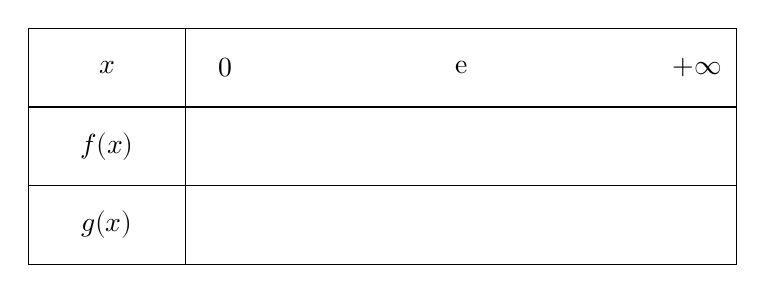
\begin{tikzpicture}
\tkzTabInit
 {$x$      /1,
  $f(x)$   /1,
  $g(x)$   /1}
 {$0$,$\E$,$+\infty$}
\end{tikzpicture}
\end{tkzexample}
Note the use of the macro \tkzcname{E} \footnote{\tkzcname{E} is defined by \BS newcommand*\{\BS E\}\{\BS ensuremath\{\BS mathrm\{e\}\}\}.}
\subsubsection{Minimal table}
\index{Minimal table}
The first argument is \tkzname{ /1}: this is the minimal argument. The argument is a list whose separator is the symbol \tkzname{/}, preceded here by a space or by nothing, so the first cell of the row is empty. \tkzname{$1$} means \tkzname{$1$ cm}: a dimension in cm is required to give the height of the row. The second argument is made of two empty elements, or of two spaces separated by a comma. This argument must contain at least two elements: the bounds of an interval.

\begin{tkzexample}[width=8cm,small]
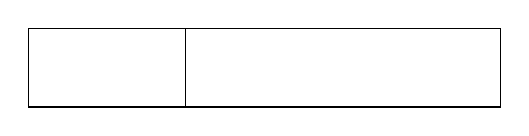
\begin{tikzpicture}
 \tkzTabInit{  / 1}
            {  ,  }
\end{tikzpicture}
\end{tkzexample}

\subsection{Using the options}

First, some dimensions of the columns can be changed. Here are the default values.

\begin{center}
  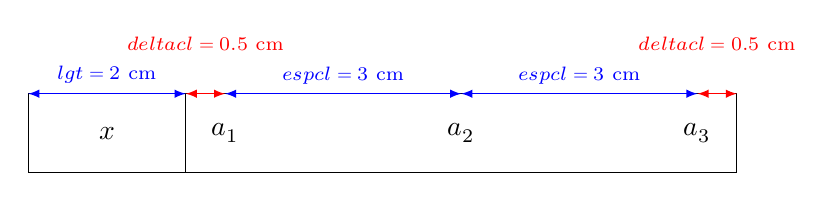
\begin{tikzpicture}
     \tkzTabInit
        {$x$ /  1}
        {$a_1$ ,  $a_2$ , $a_3$}
    \begin{scope}[arstyle/.style={>=latex,#1,<->}]
      \draw[arstyle=blue] (N10) to node[above,color=blue]%
           {\scriptsize $ espcl = 3$ cm} (N20);
      \draw[arstyle=blue] (N20) to node[above,color=blue]%
           {\scriptsize $ espcl = 3$ cm} (N30);
      \draw[arstyle=red] (T10) to node[above=12pt,color=red]%
           {\scriptsize $ deltacl = 0.5$ cm} (N10);
      \draw[arstyle=red] (N30) to node[above=12pt,color=red]%
           {\scriptsize $ deltacl = 0.5$ cm} (T20);
      \draw[arstyle=blue] (T00) to node[above,color=blue]%
           {\scriptsize $ lgt = 2$ cm} (T10);
    \end{scope}
  \end{tikzpicture}
\end{center}


\subsubsection{\texttt{\textcolor{red}{lgt}}: width of the first column}\Iopt{tkzTabInit}{lgt}

By default, the first column is $2$ cm wide. The unit is always the \tkzname{cm}.

\begin{tkzexample}[width=8cm,small]
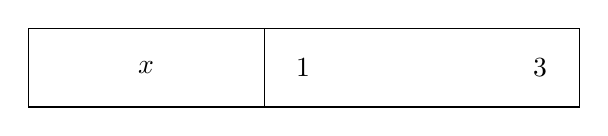
\begin{tikzpicture}
  \tkzTabInit[lgt=3]{ $x$ / 1}
                    { $1$  , $3$ }
\end{tikzpicture}
\end{tkzexample}

\subsubsection{\texttt{\textcolor{red}{espcl}}: space between two values}\Iopt{tkzTabInit}{espcl}

\begin{tkzexample}[width=9cm,small]
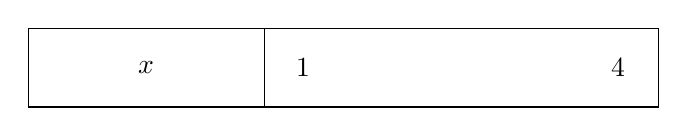
\begin{tikzpicture}
   \tkzTabInit[lgt=3,espcl=4]%
    { $x$ / 1}
    { $1$ , $4$  }
\end{tikzpicture}
\end{tkzexample}

\subsubsection{\texttt{\textcolor{red}{deltacl}}: margins at both ends}\Iopt{tkzTabInit}{deltacl}

\begin{tkzexample}[width=9cm,small]
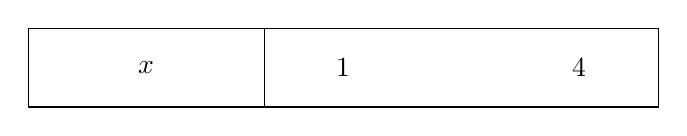
\begin{tikzpicture}
  \tkzTabInit[lgt=3,deltacl=1]%
  { $x$ / 1}
  { $1$ , $4$ }
\end{tikzpicture}
\end{tkzexample}

\subsubsection{\texttt{\textcolor{red}{lw}}: line width of the table}
\Iopt{tkzTabInit}{lw}
This is not recommended: all the lines of a document should preferably have the same width, which is $\np{0.4}$ pt by default.

\begin{tkzexample}[width=8cm,small]

\begin{tikzpicture}
  \tkzTabInit[lw=2pt]{ / 1}
                    { , }
\end{tikzpicture}
\end{tkzexample}

\subsubsection{\texttt{\textcolor{red}{nocadre}}: removing the outer frame}
\Iopt{tkzTabInit}{nocadre}

\begin{tkzexample}[width=8cm,small]
\begin{tikzpicture}
  \tkzTabInit[nocadre]{ / 1, /1, /1}
                      { , }
\end{tikzpicture}
\end{tkzexample}

\subsubsection{\texttt{\textcolor{red}{color}}: using colors in a table}
\Iopt{tkzTabInit}{color}\NamePack{amsmath}
\tkzname{color} is a boolean that says you want to use colors. You then give the colors of the first row \tkzname{colorL}, of the first column \tkzname{colorC}, of the cell of the variable \tkzname{colorV} and of the rows \tkzname{colorT}. A color can also be given to a particular row.

\tkzname{tkzTabInit\{[color]\}} means that the boolean color is true.

\begin{tkzexample}[width=8cm,small]
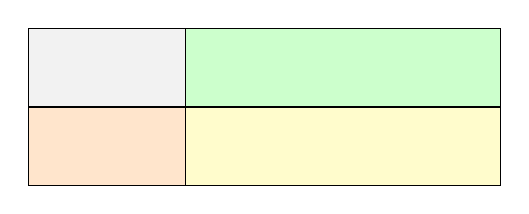
\begin{tikzpicture}
  \tkzTabInit[color,
              colorT = yellow!20,
              colorC = orange!20,
              colorL = green!20,
              colorV = lightgray!20]
             { /1 , /1}{ , }
\end{tikzpicture}
\end{tkzexample}

\begin{tkzexample}[width=8cm]
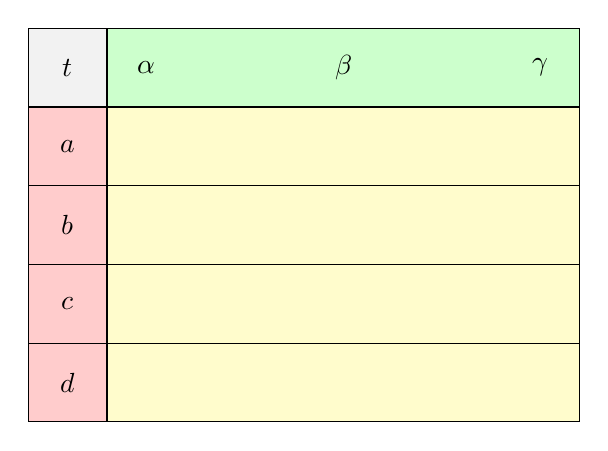
\begin{tikzpicture}
 \tkzTabInit[color,
             colorT = yellow!20,
             colorC = red!20,
             colorL = green!20,
             colorV = lightgray!20,
             lgt    = 1,
             espcl  = 2.5]%
   {$t$/1,$a$/1,$b$/1,$c$/1,$d$/1}%
   {$\alpha$,$\beta$,$\gamma$}%
\end{tikzpicture}
\end{tkzexample}

\subsubsection{\texttt{\textcolor{red}{help}}: shows the structure of the table}
\Iopt{tkzTabInit}{help}
See the section ``Customizing the tables'' (\ref{pers}).
\endinput

\newpage
\section{Creating a line of signs: \tkzcname{tkzTabLine}}
\subsection{Definition}

\begin{NewMacroBox}{tkzTabLine}{\oarg{local options}\var{s(1),...,s(2n-1)}}
  $n$ is the number of elements of the second argument of \tkzname{tkzTabInit}.

\medskip
\begin{tabular}{lll}
\toprule
symbol in an odd position &  & definition \\
\midrule
\TAline{z} {}  {draws a dotted rule with a centered zero}
\TAline{t} {}  {draws a centered dotted rule}
\TAline{d} {}  {draws a centered double bar}
\TAline{\BS textvisiblespace}{} {nothing }
\bottomrule
\end{tabular}

\medskip
\begin{tabular}{lll}
\toprule
symbol in an even position & & definition                   \\
\midrule
\TAline{h}  {}  {forbidden zone}
\TAline{+}  {}  {the sign $+$}
\TAline{-}  {}  {the sign $-$}
\TAline{\BS textvisiblespace}{} {nothing }
\bottomrule

\end{tabular}


\medskip
\noindent\emph{\tkzcname{tkzTabLine} takes as argument a list of symbols. In \tkzname{normal} use, the symbols belong to two categories: symbols in odd positions and symbols in even positions. Symbols in odd positions are usually rules, and symbols in even positions are usually ``$+$ or $-$'' signs. Symbols in odd positions act graphically: they draw vertical rules. If the second argument of \tkzcname{tkzTabInit} has \textcolor{red}{$n$} elements (values of the variable), the argument of \tkzcname{tkzTabLine} contains \tkzname{$n$} of them. Symbols in even positions give a ``$+$ or $-$'' sign or a forbidden zone (hatched or colored). Each line of signs contains \tkzname{$n-1$} of them, so it has \tkzname{$2n-1$} elements in all, that is \tkzname{$2n-2$} commas!\\
The ``recognized'' symbols are given in the tables above, but you can put almost anything. Be careful, however: the comma \textcolor{red}{(,)} is the list separator, so a decimal number written with a comma must be protected. You have several possibilities:
\begin{itemize}
\item[--] \{4,5\}: put the number between braces.
\item[--] \tkzcname{numprint\{4,5\}} or \tkzcname{np\{4,5\}}, with the excellent package \tkzname{numprint}\NamePack{numprint}, loaded with the option \tkzname{np} for the shortcut.
\end{itemize}}

\medskip
\begin{tabular}{lllc}
\toprule
options   & default       & definition         \\
\midrule
\TOline{style}  {dotted    } {style of the vertical rules               }
\TOline{help}   {no default} {shows the structure of a line of signs     }
\bottomrule
\end{tabular}

\medskip
\noindent\emph{The style of the vertical rules can be changed locally, and you can get information about the structure of the line.}
\end{NewMacroBox}

\subsection{Number of arguments}
The general syntax is:

\begin{tkzltxexample}[]
 \tkzTabInit{ e(1),...,e(i),...,e(p)} % table with p rows
            { a(1),...,a(i),...,a(n)} % n values
 \tkzTabLine{ s(1),...,s(i),...,s(2n-1)}
\end{tkzltxexample}


\medskip
If the first row has \tkzname{$n$} values, there are \tkzname{$n$} symbols in odd positions and \tkzname{$n-1$} symbols in even positions, that is \tkzname{$2n-1$} symbols.

 The main symbols are: \tkzname{z} for a zero placed on a rule, \tkzname{t} for a rule matching a zero of another row, and \tkzname{d} for a value where the expression is not defined.

A simple illustration: three values $a_1$, $a_2$ and $a_3$ allow $2\times3 -1 =5$ symbols. With $3$ values in the first row, the argument of \tkzcname{tkzTabLine} must have {$2\times 3-1=5$} elements: a list of $3$ symbols in odd positions and $2$ symbols in even positions, that is $5$ symbols separated by $4$ commas.

\begin{center}
  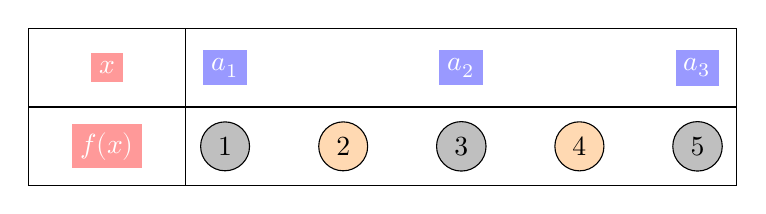
\begin{tikzpicture}
    \tkzTabInit[espcl=3,lgt=2]%
    {\colorbox{red!40}{\textcolor{white}{$x$}}    / 1,%
     \colorbox{red!40}{\textcolor{white}{$f(x)$}} / 1}%
    {\colorbox{blue!40}{\textcolor{white}{ $a_1$}},%
     \colorbox{blue!40}{\textcolor{white}{ $a_2$}},%
     \colorbox{blue!40}{\textcolor{white}{ $a_3$}}}%
    \path (N11)--(N12) node[circle,draw, fill= lightgray,midway] {1};
    \path (N12)--(N21) node[midway] {$,$};
    \path (N21)--(N22) node[circle, draw, fill= lightgray,midway] {3};
    \path (N31)--(N32) node[circle,draw,  fill= lightgray,midway] {5};
    \path (M11)--(M12) node[circle, draw, fill= orange!30,midway] {2};
    \path (M21)--(M22) node[circle,draw,  fill= orange!30,midway] {4};
  \end{tikzpicture}
\end{center}

To get this line, enter
\begin{tkzexample}[code only]\tkzTabLine{ $1$ , $2$ , $3$ , $4$ , $5$}
\end{tkzexample}


\subsection{Minimal use}
The second row is empty, but the argument of \tkzcname{tkzTabLine} must contain \tkzname{$4$} commas: it is a list of \tkzname{$5 = 2\times3-1$} values.

\begin{tkzexample}[code only]
 \tkzTabLine{,,,,} or \tkzTabLine{ , , , , }\end{tkzexample}

\begin{tkzexample}[width=8cm,small]
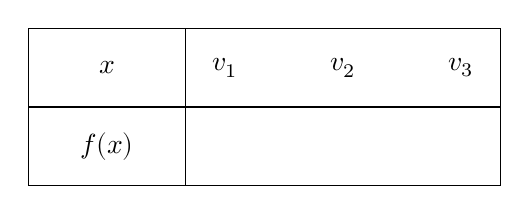
\begin{tikzpicture}
  \tkzTabInit[espcl=1.5]
     {$x$  / 1 ,$f(x)$ /1 }%
     {$v_1$ , $v_2$ , $v_3$ }%
  \tkzTabLine{ , , , , }
\end{tikzpicture}
\end{tkzexample}

\subsubsection{\texttt{\textcolor{red}{t}}: adding a rule}
This symbol draws a simple vertical rule.
\begin{tkzexample}[width=8cm,small]
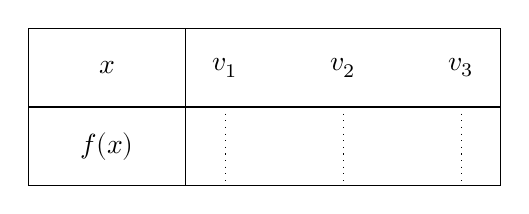
\begin{tikzpicture}
  \tkzTabInit[espcl=1.5]
     {$x$  / 1 ,$f(x)$ /1 }%
     {$v_1$ , $v_2$ , $v_3$ }%
  \tkzTabLine{ t, , t , ,t }
\end{tikzpicture}
\end{tkzexample}

\subsubsection{\texttt{\textcolor{red}{z}}: adding a zero on a vertical rule}
\begin{tkzexample}[width=8cm,small]
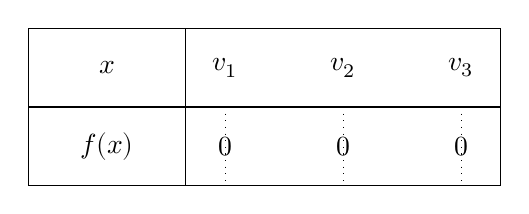
\begin{tikzpicture}
  \tkzTabInit[espcl=1.5]
     {$x$  / 1 ,$f(x)$ /1 }%
     {$v_1$ , $v_2$ , $v_3$ }%
  \tkzTabLine{ z, , z , ,z }
\end{tikzpicture}
\end{tkzexample}

\subsubsection{\texttt{\textcolor{red}{d}}: double bar}

A function may be undefined at $0$ and at $2$ and vanish at $1$. Put the symbol |d| at each end.

\begin{tkzexample}[width=7cm,small]
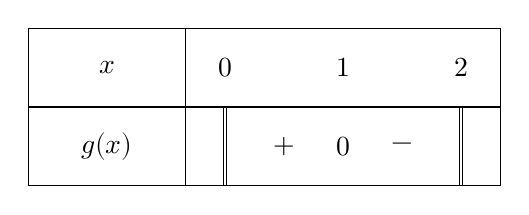
\begin{tikzpicture}
  \tkzTabInit[espcl=1.5]%
    {$x$ / 1,$g(x)$ / 1}%
    {$0$,$1$,$2$}%
\tkzTabLine{d,+,0,-,d}
\end{tikzpicture}
\end{tkzexample}

A function may also have a right derivative different from its left derivative.

\begin{tkzexample}[width=7cm,small]
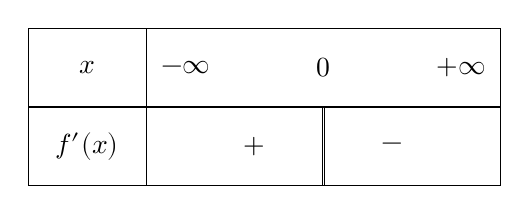
\begin{tikzpicture}
   \tkzTabInit[lgt=1.5,espcl=1.75]%
       {$x$ / 1,$f'(x)$ / 1}%
       {$-\infty$,$0$,$+\infty$}%
   \tkzTabLine{,+,d,-,}
\end{tikzpicture}
\end{tkzexample}

\subsection{Using the symbols in even positions}

In a table of signs, the symbols in even positions are normally signs, but the macro can be used in other ways. The next example shows a classic case: a zone of the table that corresponds to forbidden values. By default, with the symbol \tkzname{h}, the zone is gray, but it can be hatched if you prefer.
The last example shows how to use the macro in another way.

\subsubsection{\texttt{\textcolor{red}{h}}: forbidden zone}

A function may be undefined on an interval, here $[1, 2]$. The part of the table that corresponds to this interval is hatched or colored (by default, the zone is gray). Put |h| between the two |d| that correspond to the forbidden values\index{forbidden values} $1$ and $2$.

\begin{tkzexample}[width=8cm, small]
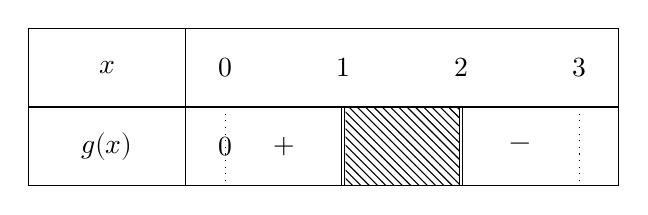
\begin{tikzpicture}
  \tkzTabInit[color,espcl=1.5]
  {$x$ / 1,$g(x)$ / 1}
  {$0$,$1$,$2$,$3$}%
  \tkzTabLine{z, + , d , h , d , - , t}
\end{tikzpicture}
\end{tkzexample}

\subsection{Using the options}

\subsubsection{\tkzname{t style}: style of the vertical rules}
\Istyle{tkzTabLine}{t style}

\begin{tkzexample}[width=7cm, small]
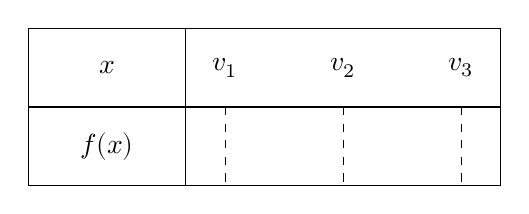
\begin{tikzpicture}
\tikzset{t style/.style = {style = dashed}}
  \tkzTabInit[espcl=1.5]
     {$x$  / 1 ,$f(x)$ /1 }%
     {$v_1$ , $v_2$ , $v_3$ }%
  \tkzTabLine{ t, , t , ,t }
\end{tikzpicture}
\end{tkzexample}


\begin{tkzexample}[width=7cm, small]
\tikzset{t style/.style = {style = densely dashed}}
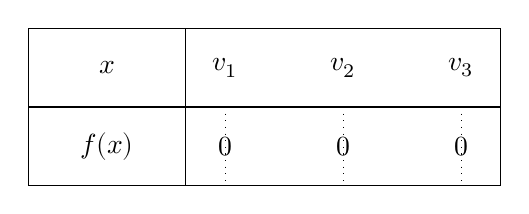
\begin{tikzpicture}
  \tkzTabInit[espcl=1.5]
     {$x$  / 1 ,$f(x)$ /1 }%
     {$v_1$ , $v_2$ , $v_3$ }%
  \tkzTabLine{ z, , z , ,z }
\end{tikzpicture}
\end{tkzexample}

\subsubsection{\tkzname{help}: shows the structure of the table}
\Iopt{tkzTabLine}{help}
See the section ``Customizing the tables'' (\ref{pers}).


\subsection{Using the styles}

\subsubsection{\tkzname{h style}: color of a forbidden zone}
\Istyle{tkzTabLine}{h style} \index{forbidden zone}
To color or hatch a zone of the table in another way, change a style.
\begin{tkzexample}[width=8cm,small]
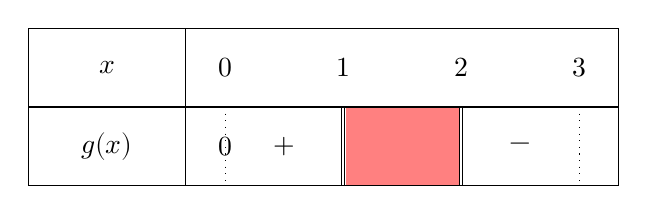
\begin{tikzpicture}
  \tikzset{h style/.style = {fill=red!50}}
  \tkzTabInit[color,espcl=1.5]%
    {$x$ / 1,$g(x)$ / 1}%
    {$0$,$1$,$2$,$3$}%
  \tkzTabLine{z,+,d,h,d,-,t}
\end{tikzpicture}
\end{tkzexample}


This time the zone is hatched.
 \index{hatching}
\begin{tkzexample}[width=8cm,small]
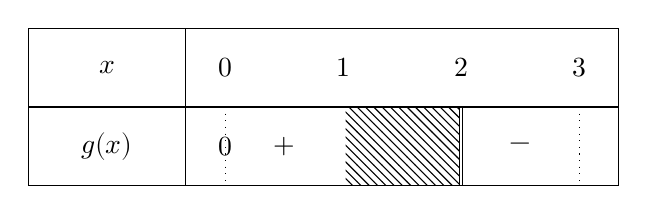
\begin{tikzpicture}
  \tikzset{h style/.style =
          {pattern=north west lines}}
  \tkzTabInit[color,espcl=1.5]%
    {$x$ / 1,$g(x)$ / 1}%
    {$0$,$1$,$2$,$3$}%
  \tkzTabLine{z,+,,h,d,-,t}
\end{tikzpicture}
\end{tkzexample}



\subsection{Examples}

\subsubsection{Simplifying an expression with an absolute value}

\begin{tkzexample}[width=8cm,small]
 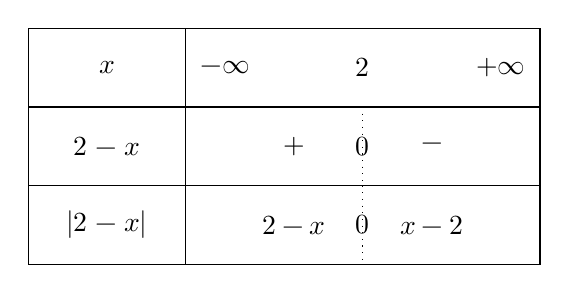
\begin{tikzpicture}
 \tkzTabInit[lgt=2,espcl=1.75]%
  {$x$/1,$2-x$/1, $\vert 2-x \vert $/1}%
  {$-\infty$,$2$,$+\infty$}%
 \tkzTabLine{ , + , z , - , }
 \tkzTabLine{ , 2-x ,z, x-2, }
\end{tikzpicture}
\end{tkzexample}

\subsubsection{Table of signs}

\begin{tkzexample}[ small]
\begin{tikzpicture}
  \tkzTabInit[lgt=3,espcl=1.5]%
     {$x$                                   /1,
      $x^2-3x+2$                            /1,
      $(x-\E)\ln x$                   /1,
      $\dfrac{x^2-3x+2}{(x-\E)\ln x}$ /2}
              {$0$  , $1$  , $2$  , $\E$  ,$+\infty$}
              \tkzTabLine{ t,+,z,-,z,+,t,+,}
              \tkzTabLine{ d,+,z,-,t,-,z,+,}
              \tkzTabLine{ d,+,d,+,z,-,d,+,}
\end{tikzpicture}
\end{tkzexample}


\subsubsection{Sign of a quadratic expression}

If $\Delta  \geq 0$, we can write $\displaystyle ax^2+bx+c=a\left(x-\dfrac{-b-\sqrt{b^2-4ac}}{2a}\right)\left(x-\dfrac{-b+\sqrt{b^2-4ac}}{2a}\right)$


\begin{tkzexample}[vbox,small]
\begin{tikzpicture}
 \tkzTabInit[color,lgt=5,espcl=3]%
   {$x$ / .8,$\Delta>0$\\ Sign of\\ $ax^2+bx+c$ /1.5}%
   {$-\infty$,$x_1$,$x_2$,$+\infty$}%
 \tkzTabLine{ , \genfrac{}{}{0pt}{0}{\text{sign of}}{a}, z
              , \genfrac{}{}{0pt}{0}{\text{opposite}}{\text{sign of}\ a}, z
              , \genfrac{}{}{0pt}{0}{\text{sign of}}{a},  }
 \end{tikzpicture}
\end{tkzexample}
 Note the use of the macro \tkzcname{genfrac}\footnote{\tkzcname{genfrac} is a macro of the package \tkzname{amsmath}}.

\medskip
If $\Delta  = 0$, we can write $\displaystyle ax^2+bx+c=a\left(x+\dfrac{b}{2a}\right)^2$

\begin{tkzexample}[vbox,width=7cm,small]
\begin{tikzpicture}
  \tkzTabInit[color,lgt=5,espcl=3]%
   {$x$ / 1 , $\Delta=0$\\ Sign of\\ $ax^2+bx+c$  / 2}%
   {$-\infty$,$\dfrac{-b}{2a}$,$+\infty$}%
  \tkzTabLine{ , \genfrac{}{}{0pt}{0}{\text{sign of}}{ a} , z
               , \genfrac{}{}{0pt}{0}{\text{sign of}}{a}, }
\end{tikzpicture}
\end{tkzexample}

If $\Delta  < 0$, then $\displaystyle ax^2+bx+c=a\left[\left(x+\dfrac{b}{2a}\right)^2 -\dfrac{b^2-4ac}{4a^2}\right]$

\begin{tkzexample}[vbox,width=7cm,small]
\begin{tikzpicture}
  \tkzTabInit[color,lgt=5,espcl=5]%
   {$x$/.8,$\Delta<0$\\ Sign of\\ $ax^2+bx+c$/2}%
   {$-\infty$,$+\infty$}%
 \tkzTabLine{ , \genfrac{}{}{0pt}{0}{\text{sign of}}{ a}, }
\end{tikzpicture}
\end{tkzexample}


\endinput

\section{Creating a line of variations: \addbs{tkzTabVar}}
\subsection{Definition}

\begin{NewMacroBox}{tkzTabVar}{\oarg{local options}\var{el($1$),\dots,el($n$)}}
  with \tkzname{el($i$) = s($i$) / e($i$)} or \tkzname{el($i$) = s($i$) / eg($i$) / ed($i$)}.

\noindent\tkzname{s($i$)} is a sequence of symbols chosen from the table below. \tkzname{eg($i$)} and \tkzname{ed($i$)} are mathematical expressions placed on the left (\emph{gauche}) and on the right (\emph{droite}) of the vertical rules. \tkzname{e($i$)} is an expression centered on a rule.

\medskip
 \begin{tabular}{llrl}
\toprule
 Group 1& \emph{with one sign} &&\\
\midrule
\tkzname{s($i$)}  & Position of the expressions & \tkzname{el($i$)}  &      \\
\midrule
\IargName{tkzTabVar}{$-~~~$}& single expression, centered, at the bottom  eg=ed   &  $-   $&$/e    $    \\
\IargName{tkzTabVar}{$+~~~$}& single expression, centered, at the top eg=ed   &  $+   $&$/e    $    \\
\IargName{tkzTabVar}{$~R~~$}& nothing, go to the next expression           &  $~R  $&$(/)   $    \\
\IargName{tkzTabVar}{$-C$}  & continuous extension at the bottom, centered &  $-C  $&$/e    $    \\
\IargName{tkzTabVar}{$+C$}  & continuous extension at the top, centered&  $+C  $&$/e    $    \\
\IargName{tkzTabVar}{$-H$}  & expression at the bottom, centered, then forbidden zone  &  $-H  $&$/e    $    \\
\IargName{tkzTabVar}{$+H$}  & expression at the top, centered, then forbidden zone &  $+H  $&$/e    $    \\
\IargName{tkzTabVar}{$+D~~$}& discontinuity, expression at the top left        &  $+D  $&$/e    $    \\
\IargName{tkzTabVar}{$-D~~$}& discontinuity, expression at the bottom left         &  $-D  $&$/e    $    \\
\IargName{tkzTabVar}{$~D+~$}& discontinuity, expression at the top right     &  $D+  $&$/e    $    \\
\IargName{tkzTabVar}{$~D-~$}& discontinuity, expression at the bottom right        &  $D-  $&$/e    $    \\
\IargName{tkzTabVar}{$+DH$} & discontinuity on the left, at the top, then forbidden zone&  $+DH $&$/e    $  \\
\IargName{tkzTabVar}{$-DH$} & discontinuity on the left, at the bottom, then forbidden zone &  $-DH $&$/e    $    \\
\IargName{tkzTabVar}{$+CH$} & continuous extension then forbidden zone    &  $+CH $&$/e    $    \\
\IargName{tkzTabVar}{$-CH$} & same, but expression at the bottom left           &  $-CH $&$/e    $    \\
\midrule
 Group 2& \emph{with two signs}& &\\
\midrule
\IargName{tkzTabVar}{$+D-$} & discontinuity,\hfill two expressions    &  $+D- $&$/eg/ed$    \\
\IargName{tkzTabVar}{$-D+$} & discontinuity, \dots \hfill      that are    &  $-D+ $&$/eg/ed$    \\
\IargName{tkzTabVar}{$+D+$} & discontinuity, \dots \hfill either on the left or on the right &$+D+ $&$/eg/ed$    \\
\IargName{tkzTabVar}{$-D-$} & discontinuity, \dots \hfill either at the top or at the bottom&$-D- $&$/eg/ed$    \\
\IargName{tkzTabVar}{$+CD+$}& continuous extension on the left and          &  $+CD+$&$/eg/ed$    \\
\IargName{tkzTabVar}{$-CD-$}& \dots \hfill  two expressions that are        &  $-CD-$&$/eg/ed$    \\
\IargName{tkzTabVar}{$+CD-$}& \dots \hfill  either on the left or on the right  &  $+CD-$&$/eg/ed$    \\
\IargName{tkzTabVar}{$-CD+$}& \dots \hfill   either at the top or at the bottom   &  $-CD+$&$/eg/ed$    \\
\IargName{tkzTabVar}{$+DC+$}& continuous extension on the right and           &  $+DC+$&$/eg/ed$    \\
\IargName{tkzTabVar}{$-DC-$}& \dots \hfill  two expressions that are          &  $-DC-$&$/eg/ed$    \\
\IargName{tkzTabVar}{$+DC-$}& \dots \hfill  either on the left or on the right      &  $+DC-$&$/eg/ed$    \\
\IargName{tkzTabVar}{$-DC+$}& \dots \hfill   either at the top or at the bottom         &  $-DC+$&$/eg/ed$    \\
\IargName{tkzTabVar}{$+V+$} & like a discontinuity but without double bar, and&  $+V+ $&$/eg/ed$    \\
\IargName{tkzTabVar}{$-V-$} & \dots \hfill  two expressions that are     &  $-V- $&$/eg/ed$    \\
\IargName{tkzTabVar}{$+V-$} & \dots \hfill  either on the left or on the right &  $+V- $&$/eg/ed$    \\
\IargName{tkzTabVar}{$-V+$} & \dots \hfill   either at the top or at the bottom    &  $-V+ $&$/eg/ed$    \\
\midrule
\tkzname{\textvisiblespace} & leaves the place empty in some cases& &   \\
\bottomrule
\end{tabular}

\medskip
\noindent\emph{The macro \tkzcname{tkzTabVar} takes one argument: a list. This list has \tkzname{$n$} elements, matching the \tkzname{$n$} values of the first row. Each element gives the position of one or two expressions in the row: a sign $+$ (at the top) or a sign $-$ (at the bottom). These expressions are values of the function or limits.}

\noindent\emph{The elements \tkzname{el($i$)} have the form:\\
 either \mbox{\tkzname{\{ s($i$)/ e($i$)\}}} or \mbox{\tkzname{\{ s($i$)/ e($i$) / \}}}, or \mbox{\tkzname{\{ s($i$)/ eg($i$) / ed($i$)\}}}.}

\noindent\emph{The first form is for the symbols that have only one sign \tkzname{$+$} or \tkzname{$-$} and place a single expression; the second is for the symbols that have two signs and place two expressions. The expressions are values taken by the function on the left \tkzname{eg($i$)} or on the right \tkzname{ed($i$)}, or limits; they can also be empty. A sign \tkzname{$+$} or \tkzname{$-$} on the left (resp. on the right) of the symbol corresponds to \tkzname{eg($i$)} (resp. \tkzname{ed($i$)}).}

\medskip
\begin{tabular}{lllc}
\toprule
\texttt{options}               & \texttt{default} & \texttt{definition}              \\
\midrule
\IoptName{tkzTabVar}{color}  & |black|         & color of the arrows                \\
\IoptName{tkzTabVar}{help}   & |false| & shows the structure of a line of variations      \\
 \bottomrule
\end{tabular}

\end{NewMacroBox}

 \medskip
A picture is sometimes better than a long speech\dots

 \begin{center}
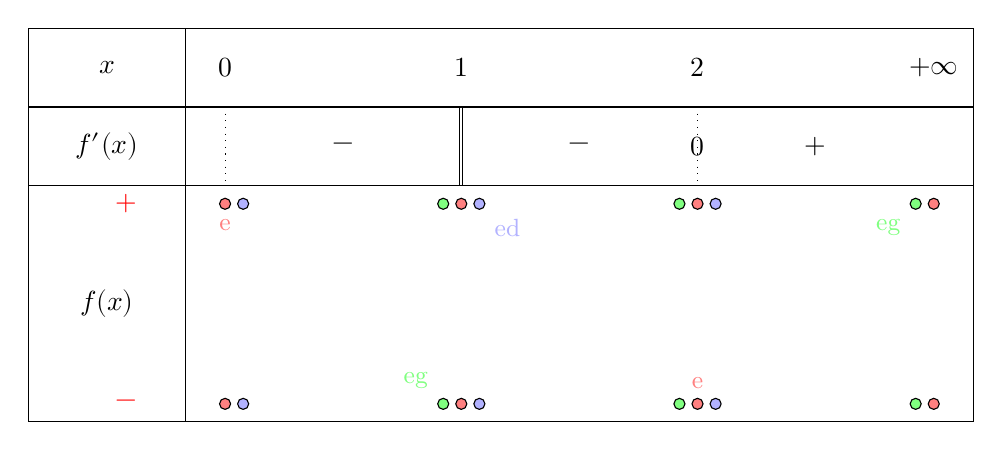
\begin{tikzpicture}
\tkzTabInit[lgt=2,espcl=3]{$x$/1,$f'(x)$/1,$f(x)$/3}%
{$0$,$1$,$2$,$+\infty$}%
\tkzTabLine{t,-,d,-,z,+,}%
\tkzTabVar{}%
\node[below =3pt]  (FN12) at (N12){};
\node[below =3pt]  (FN22) at (N22){};
\node[below =3pt]  (FN32) at (N32){};
\node[below =3pt]  (FN42) at (N42){};

\node[above =3pt]  (FN13) at (N13){};
\node[above =3pt]  (FN23) at (N23){};
\node[above =3pt]  (FN33) at (N33){};
\node[above =3pt]  (FN43) at (N43){};

\node[below right=3pt]  (FRN12) at (N12){};
\node[below right=3pt]  (FRN22) at (N22){};
\node[below right=3pt]  (FRN32) at (N32){};
\node[below right=3pt]  (FRN42) at (N42){};

\node[above right=3pt]  (FRN13) at (N13){};
\node[above right=3pt]  (FRN23) at (N23){};
\node[above right=3pt]  (FRN33) at (N33){};

\node[below left=3pt]  (FLN22) at (N22){};
\node[below left=3pt]  (FLN32) at (N32){};
\node[below left=3pt]  (FLN42) at (N42){};

\node[above left=3pt]  (FLN13) at (N13){};
\node[above left=3pt]  (FLN23) at (N23){};
\node[above left=3pt]  (FLN33) at (N33){};
\node[above left=3pt]  (FLN43) at (N43){};

\draw[fill=red!50] (FN12) circle(2pt)  node[below=2pt,text=red!50] {\small e} node[left=1cm,red] {$+$};
\draw[fill=red!50] (FN22) circle(2pt);
\draw[fill=red!50] (FN32) circle(2pt);
\draw[fill=red!50] (FN42) circle(2pt);

\draw[fill=red!50] (FN13) circle(2pt)  node[left=1cm,red] {$-$};
\draw[fill=red!50] (FN23) circle(2pt);
\draw[fill=red!50] (FN33) circle(2pt) node[above=2pt,text=red!50] {\small e};
\draw[fill=red!50] (FN43) circle(2pt);

\draw[fill=blue!30] (FRN12) circle(2pt);
\draw[fill=blue!30] (FRN22) circle(2pt) node[below right=2pt,text=blue!30] {\small ed};
\draw[fill=blue!30] (FRN32) circle(2pt);
\draw[fill=blue!30] (FRN13) circle(2pt);
\draw[fill=blue!30] (FRN23) circle(2pt);
\draw[fill=blue!30] (FRN33) circle(2pt);

\draw[fill=green!50] (FLN22) circle(2pt);
\draw[fill=green!50] (FLN32) circle(2pt);
\draw[fill=green!50] (FLN42) circle(2pt) node[below left =2pt,text=green!50] {\small eg};
\draw[fill=green!50] (FLN23) circle(2pt) node[above left =2pt,text=green!50] {\small eg};
\draw[fill=green!50] (FLN33) circle(2pt);
\draw[fill=green!50] (FLN43) circle(2pt);
\end{tikzpicture}
\end{center}

\medskip
For some of the tables, I used the following macros:

\begin{tkzexample}[code only]
	\newcommand*{\va}{\colorbox{red!50}    {$\scriptscriptstyle V_a$}}
	\newcommand*{\vb}{\colorbox{blue!50}   {$\scriptscriptstyle V_b$}}
	\newcommand*{\vbo}{\colorbox{blue!50}  {$\scriptscriptstyle V_{b1}$}}
	\newcommand*{\vbt}{\colorbox{yellow!50}{$\scriptscriptstyle V_{b2}$}}
	\newcommand*{\vc}{\colorbox{gray!50}   {$\scriptscriptstyle V_c$}}
	\newcommand*{\vd}{\colorbox{magenta!50}{$\scriptscriptstyle V_d$}}
	\newcommand*{\ve}{\colorbox{orange!50} {$\scriptscriptstyle V_e$}}
\end{tkzexample}

\medskip
 \begin{center}
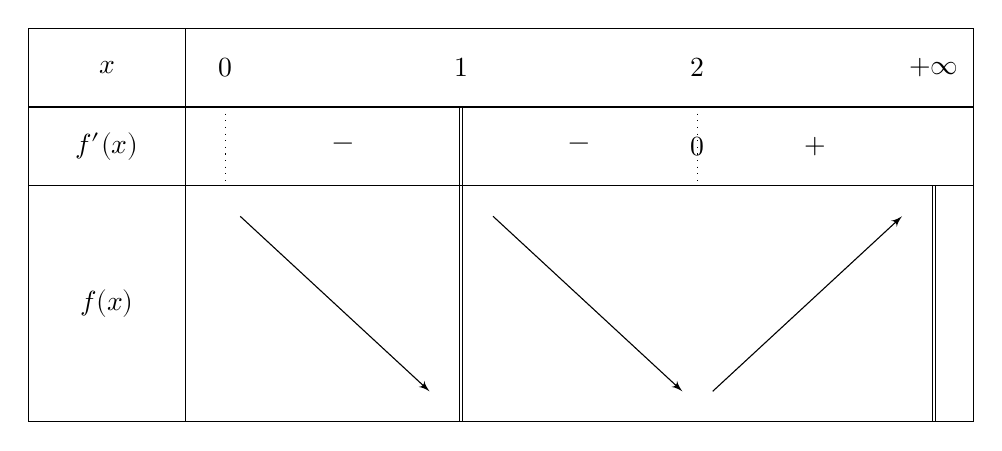
\begin{tikzpicture}
\tkzTabInit[lgt=2,espcl=3]{$x$/1,$f'(x)$/1,$f(x)$/3}%
{$0$,$1$,$2$,$+\infty$}%
  \tkzTabLine{t,-,d,-,z,+,}%
	\tkzTabVar{+/\va , -D+/\vb/\vc,-/\vd, +D/\ve}%
\end{tikzpicture}
\end{center}

\begin{tkzexample}[code only]
	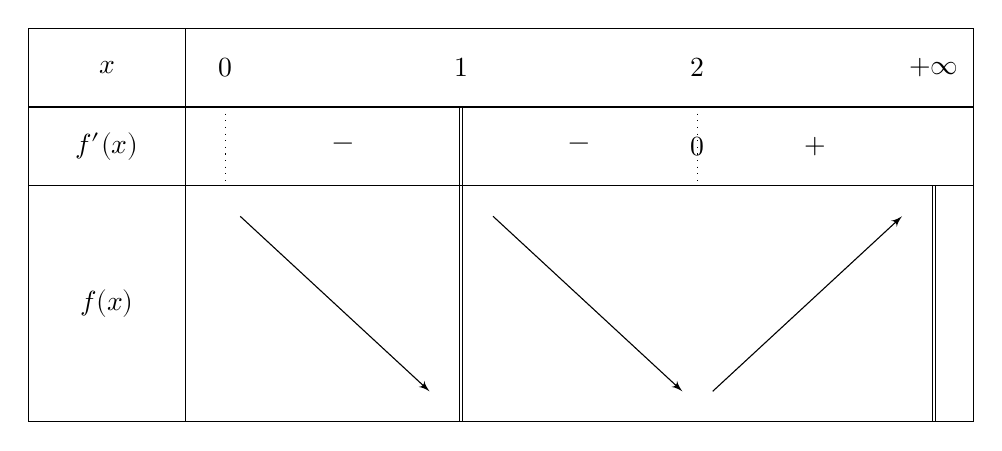
\begin{tikzpicture}
	\tkzTabInit[lgt=2,espcl=3]{$x$/1,$f'(x)$/1,$f(x)$/3}%
	{$0$,$1$,$2$,$+\infty$}%
\tkzTabLine{t,-,d,-,z,+,}%
	\tkzTabVar{+/\va , -D+/\vb/\vc,-/\vd, +D/\ve}%
\end{tikzpicture}
\end{tkzexample}

Comments: the signs $+$ and $-$ place an end of the arrow at the top or at the bottom of the row. With a single sign, a single expression is needed. Its position with respect to the column is given by the position of the sign with respect to the other symbols (see \tkzname{$+D$}). \tkzname{$-D+$} needs two expressions.

\subsection{Using the symbols}

\medskip
\bgroup\parindent=0pt
\begin{minipage}{7cm}
\begin{tkzexample}[code only]
 {+ /\va , -/\vb }
\end{tkzexample}
  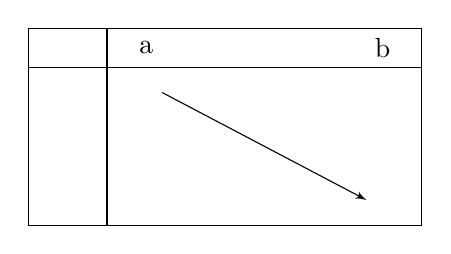
\begin{tikzpicture}
  \tkzTabInit[lgt=1]{ /0.5,/2 }{ a , b }
  \tkzTabVar%
  {+ /\va , -/\vb }
  \end{tikzpicture}
\end{minipage}
\hfill
\begin{minipage}{7cm}
\begin{tkzexample}[code only]
 {-/\va   ,   +/\vb}
\end{tkzexample}
  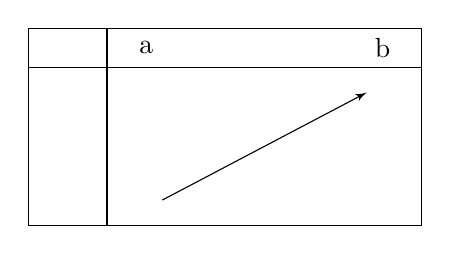
\begin{tikzpicture}
  \tkzTabInit[lgt=1]{ /0.5,/2 }{ a , b }
  \tkzTabVar%
{-/\va   ,   +/\vb}
  \end{tikzpicture}
\end{minipage}

\begin{minipage}{7cm}
\begin{tkzexample}[code only]
 {+/\va   ,   +/\vb}
\end{tkzexample}
  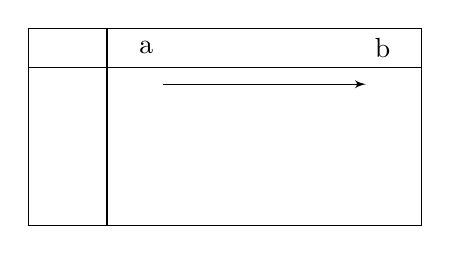
\begin{tikzpicture}
  \tkzTabInit[lgt=1]{ /0.5,/2 }{ a , b }
  \tkzTabVar%
{+/\va   ,   +/\vb}
  \end{tikzpicture}
\end{minipage}
\hfill
\begin{minipage}{7cm}
\begin{tkzexample}[code only]
 {-/\va   ,   -/\vb}
\end{tkzexample}
  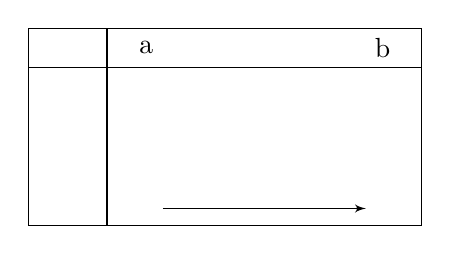
\begin{tikzpicture}
  \tkzTabInit[lgt=1]{ /0.5,/2 }{ a , b }
  \tkzTabVar%
{-/\va   ,   -/\vb}
  \end{tikzpicture}
\end{minipage}

\begin{minipage}{7cm}
\begin{tkzexample}[code only]
 {+/\va  , -C / \vb}
\end{tkzexample}
  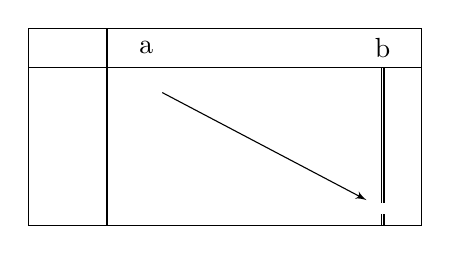
\begin{tikzpicture}
  \tkzTabInit[lgt=1]{ /0.5,/2 }{ a , b }
  \tkzTabVar%
{+/\va  , -C / \vb}
  \end{tikzpicture}
\end{minipage}
\hfill
\begin{minipage}{7cm}
\begin{tkzexample}[code only]
{-/\va  , +C / \vb }\end{tkzexample}
  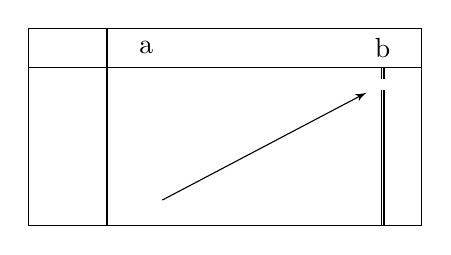
\begin{tikzpicture}
  \tkzTabInit[lgt=1]{ /0.5,/2 }{ a , b }
  \tkzTabVar%
{-/\va  , +C / \vb }
  \end{tikzpicture}
\end{minipage}

\begin{minipage}{7cm}
\begin{tkzexample}[code only]
 {+C  / \va ,  -C / \vb}
\end{tkzexample}
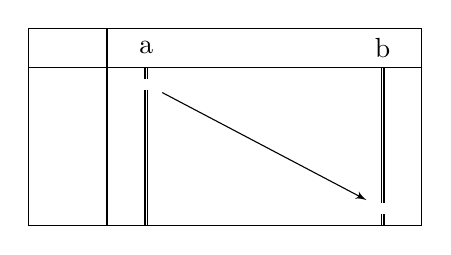
\begin{tikzpicture}
  \tkzTabInit[lgt=1]{ /0.5,/2 }{ a , b }
   \tkzTabVar%
 {+C  / \va ,  -C / \vb }
\end{tikzpicture}
\end{minipage}
\hfill
\begin{minipage}{7cm}
\begin{tkzexample}[code only]
 {-C /\va  , +C /\vb}
\end{tkzexample}
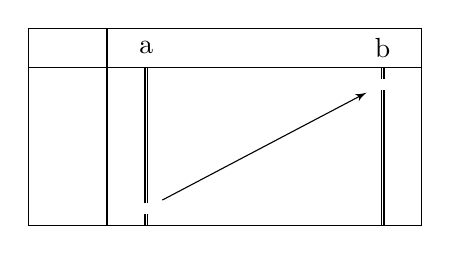
\begin{tikzpicture}
  \tkzTabInit[lgt=1]{ /0.5,/2 }{ a , b }
     \tkzTabVar%
 {-C /\va  , +C /\vb}
\end{tikzpicture}
\end{minipage}

\begin{minipage}{7cm}
\begin{tkzexample}[code only]
 { D+  /\va  ,  -/\vb}
\end{tkzexample}
  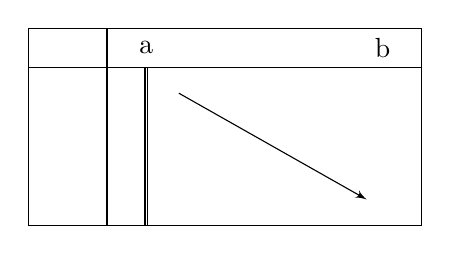
\begin{tikzpicture}
  \tkzTabInit[lgt=1]{ /0.5,/2 }{ a , b }
  \tkzTabVar%
 { D+  /\va  ,  -/\vb}
  \end{tikzpicture}
\end{minipage}
\hfill
\begin{minipage}{7cm}
\begin{tkzexample}[code only]
 { D-  /\va  ,  +/\vb}
\end{tkzexample}
  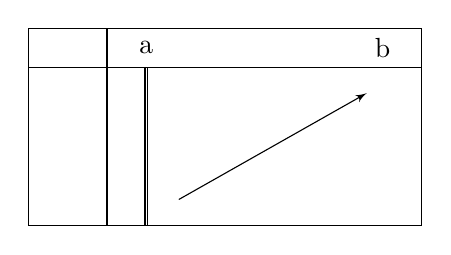
\begin{tikzpicture}
  \tkzTabInit[lgt=1]{ /0.5,/2 }{ a , b }
  \tkzTabVar
  { D-  /\va  ,  +/\vb}
  \end{tikzpicture}
\end{minipage}

\begin{minipage}{7cm}
\begin{tkzexample}[code only]
 {+/\va  , -D / \vb}
\end{tkzexample}
  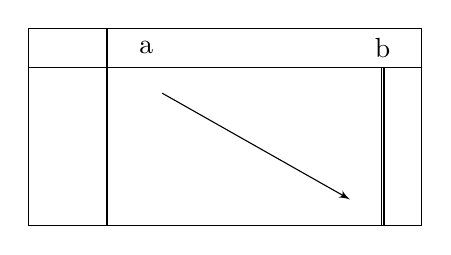
\begin{tikzpicture}
  \tkzTabInit[lgt=1]{ /0.5,/2 }{ a , b }
  \tkzTabVar%
{+/\va  , -D / \vb}
  \end{tikzpicture}
\end{minipage}
\hfill
\begin{minipage}{7cm}
\begin{tkzexample}[code only]
 {-/\va  , +D / \vb }
\end{tkzexample}
  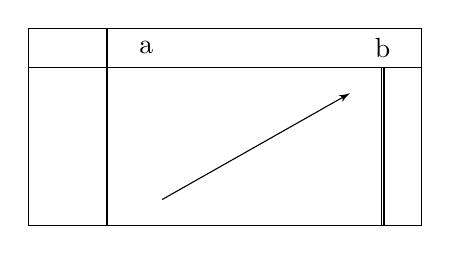
\begin{tikzpicture}
  \tkzTabInit[lgt=1]{ /0.5,/2 }{ a , b }
  \tkzTabVar%
{-/\va  , +D / \vb }
  \end{tikzpicture}
\end{minipage}

\begin{minipage}{7cm}
\begin{tkzexample}[code only]
 {D+ / \va , -D / \vb }
\end{tkzexample}
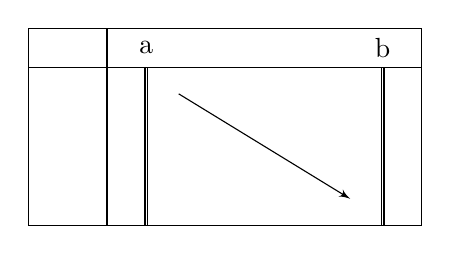
\begin{tikzpicture}
  \tkzTabInit[lgt=1]{ /0.5,/2 }{ a , b }
   \tkzTabVar%
 {D+  / \va ,  -D / \vb }
\end{tikzpicture}
\end{minipage}
\hfill
\begin{minipage}{7cm}
\begin{tkzexample}[code only]
 {D- /\va , +D /\vb}
\end{tkzexample}
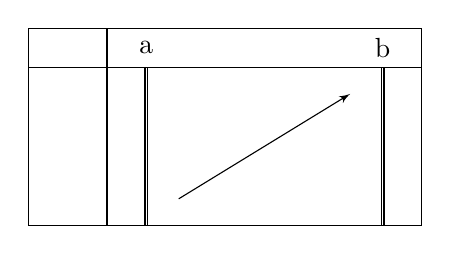
\begin{tikzpicture}
  \tkzTabInit[lgt=1]{ /0.5,/2 }{ a , b }
     \tkzTabVar%
 {D- /\va  , +D /\vb}
\end{tikzpicture}
\end{minipage}

\begin{minipage}{7cm}
\begin{tkzexample}[code only]
 {+/ \va , -/ \vb , +/ \vc}
\end{tkzexample}
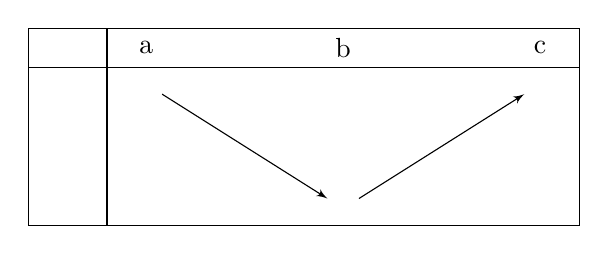
\begin{tikzpicture}
\tkzTabInit[lgt=1,espcl=2.5]{ /0.5,/2 }{ a , b , c }
\tkzTabVar  {+/ \va , -/  \vb ,+/  \vc}
\end{tikzpicture}
\end{minipage}
\hfill
\begin{minipage}{7cm}
\begin{tkzexample}[code only]
 {+/ \va ,-C/ \vb , +/  \vc/ }
\end{tkzexample}
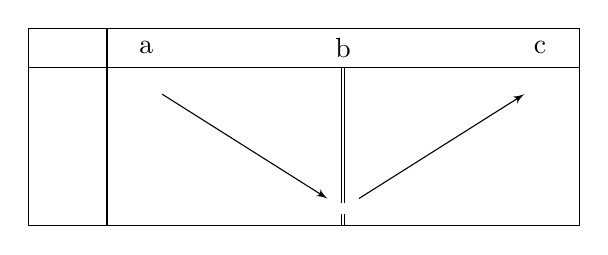
\begin{tikzpicture}
\tkzTabInit[lgt=1,espcl=2.5]{ /0.5,/2 }{ a , b , c }
\tkzTabVar {+/ \va  ,-C/ \vb , +/  \vc/ }
\end{tikzpicture}
\end{minipage}

\begin{minipage}{7cm}
\begin{tkzexample}[code only]
 {-  /\va , R , +/\vc}
\end{tkzexample}
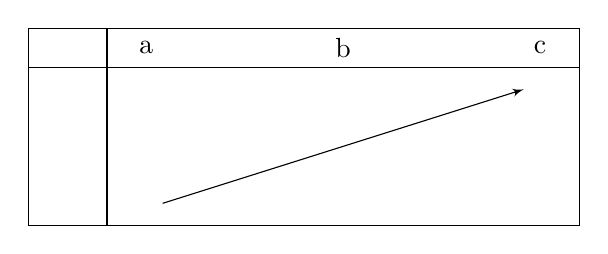
\begin{tikzpicture}
\tkzTabInit[lgt=1,espcl=2.5]{ /0.5,/2 }{ a , b , c }
\tkzTabVar%
{-  /\va  ,  R,  +/\vc}
\end{tikzpicture}
\end{minipage}
\hfill
\begin{minipage}{7cm}
\begin{tkzexample}[code only]
 {-  /\va , R , +/\vc}
\end{tkzexample}
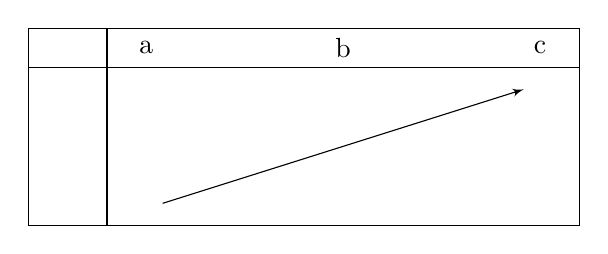
\begin{tikzpicture}
\tkzTabInit[lgt=1,espcl=2.5]{ /0.5,/2}{ a , b , c }
\tkzTabVar%
{-  /\va  ,  R  ,  +/\vc}
\end{tikzpicture}
\end{minipage}

\begin{minipage}{7cm}
\begin{tkzexample}[code only]
 {D-/\va , +DH/\vbo/ , }
\end{tkzexample}
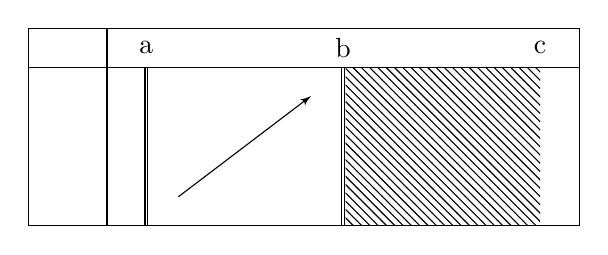
\begin{tikzpicture}
\tkzTabInit[lgt=1,espcl=2.5]{ /0.5,/2 }{ a , b , c }
\tkzTabVar%
{D-/\va  ,  +DH/\vbo/ ,  }
\end{tikzpicture}
\end{minipage}
\hfill
\begin{minipage}{7cm}
\begin{tkzexample}[code only]
 {D-/\va  , -DH/\va/\vb ,  D+/}
\end{tkzexample}
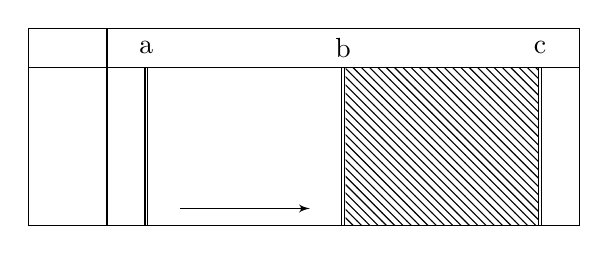
\begin{tikzpicture}
\tkzTabInit[lgt=1,espcl=2.5]{ /0.5,/2 }{ a , b , c }
\tkzTabVar%
{D-/\va  ,  -DH/\vbo ,  D+/}
\end{tikzpicture}
\end{minipage}

\begin{minipage}{7cm}
\begin{tkzexample}[code only]
 {D-/\va , +D-/\vbo/\vbt , +D/\vc}
\end{tkzexample}
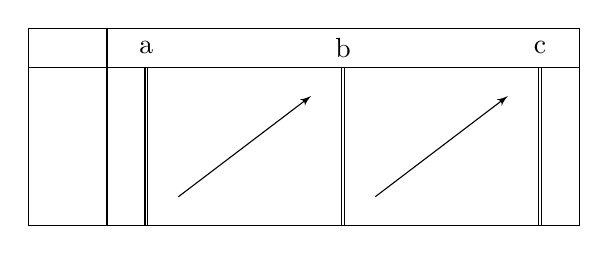
\begin{tikzpicture}
\tkzTabInit[lgt=1,espcl=2.5]{ /0.5,/2 }{ a , b , c }
\tkzTabVar%
{D-/\va  ,  +D-/\vbo/\vbt , +D/\vc}
\end{tikzpicture}
\end{minipage}
\hfill
\begin{minipage}{7cm}
\begin{tkzexample}[code only]
 {D-/\va , +D-/\vbo/\vbt , +D/\vc}
\end{tkzexample}
\begin{tikzpicture}
\tkzTabInit[lgt=1,espcl=2.5]{ /0.5,/2 }{ a , b , c }
\tkzTabVar%
{D-/\va  ,  -D-/\vbo/\vbt , +D/\vc}
\end{tikzpicture}
\end{minipage}

\begin{minipage}{7cm}
\begin{tkzexample}[code only]
 {+/\va , -D- / \vbo/\vbt , +/\vc}
\end{tkzexample}
\begin{tikzpicture}
\tkzTabInit[lgt=1,espcl=2.5]{ /0.5,/2 }{ a , b , c }
\tkzTabVar  {+/ \va , -D- /\vbo/\vbt,+/\vc  }
\end{tikzpicture}
\end{minipage}
\hfill
\begin{minipage}{7cm}
\begin{tkzexample}[code only]
 {+ /\va,-DC- /\vbo/\vbt,+ /\vc}
\end{tkzexample}
\begin{tikzpicture}\tikzset{low/.style   = {above  =  15pt}}
\tkzTabInit[lgt=1,espcl=2.5]{ /0.5,/2 }{ a , b , c }
\tkzTabVar {+   /\va ,-DC- /\vbo/\vbt  ,+ /\vc}
\end{tikzpicture}
\end{minipage}

\begin{minipage}{7cm}
\begin{tkzexample}[code only]
 {D-/\va, +DC-/\vbo/\vbt, +D/\vc}
\end{tkzexample}
\begin{tikzpicture}
\tkzTabInit[lgt=1,espcl=2.5]{ /0.5,/2 }{ a , b , c }
\tkzTabVar%
{D-/\va  ,  +DC-/\vbo/\vbt ,+D/\vc}
\end{tikzpicture}
\end{minipage}
\hfill
\begin{minipage}{7cm}
\begin{tkzexample}[code only]
 {D+/\va , +DC-/\vbo/\vbt , +D/\vc}
\end{tkzexample}
\begin{tikzpicture}
\tkzTabInit[lgt=1,espcl=2.5]{ /0.5,/2 }{ a , b , c }
\tkzTabVar%
{D+/\va  ,  +DC-/\vbo/\vbt ,+D/\vc}
\end{tikzpicture}
\end{minipage}

\begin{minipage}{7cm}
\begin{tkzexample}[code only]
 {D-/\va , +CD-/\vbo/\vbt , +D/\vc}
\end{tkzexample}
\begin{tikzpicture}
\tkzTabInit[lgt=1,espcl=2.5]{ /0.5,/2 }{ a , b , c }
\tkzTabVar%
{D-/\va  ,  +CD-/\vbo/\vbt , +D/\vc}
\end{tikzpicture}
\end{minipage}
\hfill
\begin{minipage}{7cm}
\begin{tkzexample}[code only]
 {D-/\va , +CD-/\vbo/\vbt ,+D/\vc}
\end{tkzexample}
\begin{tikzpicture}
\tkzTabInit[lgt=1,espcl=2.5]{ /0.5,/2 }{ a , b , c }
\tkzTabVar%
{D+/\va , +CD-/\vbo/\vbt ,  +D/\vc}
\end{tikzpicture}
\end{minipage}

\begin{minipage}{7cm}
\begin{tkzexample}[code only]
 {+/\va, -DC+ /\vbo/\vbt, - /\vc}
\end{tkzexample}
\begin{tikzpicture}
\tkzTabInit[lgt=1,espcl=2.5]{ /0.5,/2 }{ a , b , c }
\tkzTabVar  {+ /\va ,-DC+ /\vbo/\vbt , -/\vc}
\end{tikzpicture}
\end{minipage}
\hfill
\begin{minipage}{7cm}
\begin{tkzexample}[code only]
 {D- /\va, -DC- /\vbo/\vbt,+D/\vc}
\end{tkzexample}
\begin{tikzpicture}\tikzset{low/.style           = {above       =  15pt}}
\tkzTabInit[lgt=1,espcl=2.5]{ /0.5,/2 }{ a , b , c }
\tkzTabVar%
{D- /\va  , -DC- /\vbo/\vbt , +D/\vc}
\end{tikzpicture}
\end{minipage}

\begin{minipage}{7cm}
\begin{tkzexample}[code only]
 {+/\va  , -CH /\vbo/\vbt , D+/}
\end{tkzexample}
\begin{tikzpicture}
\tkzTabInit[lgt=1,espcl=2.5]{ /0.5,/2 }{ a , b , c }
\tkzTabVar%
{+/\va  , -CH /\vbo/\vbt , D+/}
\end{tikzpicture}
\end{minipage}
\hfill
\begin{minipage}{7cm}
\begin{tkzexample}[code only]
 {+  /\va  , -CH/\vb,  //}
\end{tkzexample}
\begin{tikzpicture}
\tkzTabInit[lgt=1,espcl=2.5]{ /0.5,/2 }{ a , b , c }
\tkzTabVar%
{+  /\va  , -CH/\vb,  //}
\end{tikzpicture}
\end{minipage}

\begin{minipage}{7cm}
\begin{tkzexample}[code only]
 {+/\va , -V- /\vbo /\vbt, +/\vc}
\end{tkzexample}
\begin{tikzpicture}
\tkzTabInit[lgt=1,espcl=2.5]{ /0.5,/2 }{ a , b , c }
\tkzTabVar  {+/\va,-V- /\vbo /\vbt, +/\vc}
\end{tikzpicture}
\end{minipage}
\hfill
\begin{minipage}{7cm}
\begin{tkzexample}[code only]
 {+/ \va ,-V+ / \vbo/ \vbt ,-/ \vc}
\end{tkzexample}
\begin{tikzpicture}
\tkzTabInit[lgt=1,espcl=2.5]{ /0.5,/2 }{ a , b , c }
\tkzTabVar  {+/ \va ,-V+ / \vbo/ \vbt ,-/ \vc}
\end{tikzpicture}
\end{minipage}

\begin{minipage}{7cm}
\begin{tkzexample}[code only]
 {+/ \va ,+V- /\vbo/ \vbt , -/\vc}
\end{tkzexample}
\begin{tikzpicture}
\tkzTabInit[lgt=1,espcl=2.5]{ /0.5,/2 }{ a , b , c }
\tkzTabVar  {+/ \va ,+V- / \vbo/ \vbt , -/\vc}
\end{tikzpicture}
\end{minipage}
\hfill
\begin{minipage}{7cm}
\begin{tkzexample}[code only]
 {-/ \va, +V+ / \vbo/\vbt, -/\vc}
\end{tkzexample}
\begin{tikzpicture}
\tkzTabInit[lgt=1,espcl=2.5]{ /0.5,/2 }{ a , b , c }
\tkzTabVar  {-/ \va ,+V+ / \vbo / \vbt, -/\vc}
\end{tikzpicture}
\end{minipage}

\begin{minipage}{16cm}
\begin{tkzexample}[code only]
 {-/ \va ,+H/\vb,-/\vc, +/ \vd}
\end{tkzexample}
\begin{tikzpicture}
\tkzTabInit[lgt=1,espcl=3]{ /0.5,/2 }{ a , b , c , d }
\tkzTabVar  {-/  \va  ,+H/\vb,-/\vc, +/  \vd}
\end{tikzpicture}
\end{minipage}

\begin{minipage}{16cm}
\begin{tkzexample}[code only]
 {+/  \va  ,-H/\vb,-/\vc, +/  \vd}
\end{tkzexample}
\begin{tikzpicture}
\tkzTabInit[lgt=1,espcl=3]{ /0.5,/2 }{ a , b , c , d }
\tkzTabVar  {+/  \va  ,-H/\vb,-/\vc, +/  \vd}
\end{tikzpicture}
\end{minipage}

\begin{minipage}{16cm}
\begin{tkzexample}[code only]
 {-/  \va  , R , R , R , +/  \ve}
\end{tkzexample}
\begin{tikzpicture}
\tkzTabInit[lgt=1,espcl=3]{ /0.5,/2 }{ a , b , c , d , e}
\tkzTabVar  {-/  \va  ,R,R,R, +/  \ve}
\end{tikzpicture}
\end{minipage}

\begin{minipage}{16cm}
\begin{tkzexample}[code only]
  {-/ \va , +/\vb , -DH/\vc , -/\vd , +/ \ve}
 \end{tkzexample}
\begin{tikzpicture}
\tkzTabInit[lgt=1,espcl=3]{ /0.5,/2 }{ a , b , c , d , e}
\tkzTabVar  {-/ \va  ,+/\vb ,-DH/\vc,-/\vd, +/ \ve}
\end{tikzpicture}
\end{minipage}

\begin{minipage}{16cm}
\begin{tkzexample}[code only]
 {D-/ \va , +DH/\vb/ , D-/\vc , +/\vd , +D/\ve}
\end{tkzexample}
\begin{tikzpicture}
\tkzTabInit[lgt=1,espcl=3]{ /0.5,/2 }{ a , b , c , d , e}
\tkzTabVar  {D-/  \va ,+DH/\vb/,D-/\vc,+/\vd, -D/\ve}
\end{tikzpicture}
\end{minipage}
\egroup

\medskip
Comments
\begin{itemize}
  \item the syntax $s(i)/\ldots/\ldots$ can be used in almost every case, but then the expressions must be placed correctly;

  \item the empty argument is sometimes used at the end of a row, but then no arrow is drawn;

  \item $C+$ and $C-$ do not exist: $+C$ and $-C$ are enough because the expressions are centered;
  \item $D+$ and $D-$ do exist.

\end{itemize}


\subsection{Using the options}

\subsubsection{\texttt{\textcolor{red}{color}}: color of the arrows}
The table can be customized with styles.
\begin{tkzexample}[vbox, small]
\begin{tikzpicture}
  \tkzTabInit[color,espcl=8]%
    {$x$   /1,%
     Sign\\ of $\dfrac{1}{x}$ /1.5,
     Variations\\ of $\ln$      /1.5}%
    {$0$,$+\infty$}%
  \tkzTabLine{d,+,}%
  \tkzTabVar[color=red]%
    {D-/    /  $-\infty$,+/  $+\infty$  /}
\end{tikzpicture}
\end{tkzexample}

\subsubsection{\texttt{\textcolor{red}{help}}: shows the structure of the table}
\Iopt{tkzTabVar}{help}
See the section ``Customizing the tables'' (\ref{pers}).
\subsection{Using the styles}

\subsubsection{Color of a forbidden zone}
\Istyle{tkzTabvar}{h style}
To color or hatch a zone of the table in another way, change a style.

By default, \tkzname{h style} is defined as follows:
\begin{tkzexample}[code only]
 \tikzset{h style/.style = {fill=gray,opacity=0.4}}
\end{tkzexample}

Another definition could be:

\begin{tkzexample}[code only]
 \tikzset{h style/.style = {fill=red!50}}
\end{tkzexample}

\begin{tkzexample}[vbox,width=9cm]
\begin{tikzpicture}
 \tikzset{h style/.style = {fill=red!50}}
 \tkzTabInit[lgt=1,espcl=2]{$x$ /1,  $f$ /2}{$0$,$1$,$2$,$3$}%
 \tkzTabVar{+/ $1$  / , -CH/ $-2$ / , +C/  $5$, -/ $0$  /  }
\end{tikzpicture}
\end{tkzexample}

\subsubsection{\texttt{\textcolor{red}{h style}}: hatched forbidden zone}
\Istyle{tkzTabVar}{h style}

\begin{tkzexample}[code only]
  \tikzset{h style/.style = {pattern=north west lines}}
\end{tkzexample}
 This code hatches the zone.

\begin{tkzexample}[vbox,width=9cm,small]
\begin{tikzpicture}
 \tikzset{h style/.style = {pattern=north west lines}}
 \tkzTabInit[lgt=1,espcl=2]{$x$ /1,  $f$ /2}{$0$,$1$,$2$,$3$}%
 \tkzTabVar{+/ $1$  / , -CH/ $-2$ / , +C/  $5$, -/ $0$  /  }
\end{tikzpicture}
\end{tkzexample}


\subsubsection{\texttt{\textcolor{red}{arrow style}}: style of the arrows}
\Istyle{tkzTabVar}{arrow}
The style of the arrows is \tkzname{arrow style}; it is defined as follows:

\begin{tkzexample}[code only]
   \tikzset{arrow style/.style   = {\cmdTAB@VA@color,
                                    ->,
                                    >           = latex',
                                    shorten >   =  2pt,
                                    shorten <   =  2pt}}
\end{tkzexample}

 The arrows stop short of the nodes. Here is a possible change of the style:

\begin{tkzexample}[code only]
  \tikzset{arrow style/.style   = {blue,
                                   ->,
                                   >           = latex',
                                   shorten >   =  6pt,
                                   shorten <   =  6pt}}
\end{tkzexample}

 The color of the arrows and the gap at their ends are changed.

\begin{tkzexample}[vbox,small]
\begin{tikzpicture}
  \tikzset{arrow style/.style   = {blue,
                                   ->,
                                   >           = latex',
                                   shorten >   =  6pt,
                                   shorten <   =  6pt}}
  \tkzTabInit[espcl=5]{$x$ /1, $\ln x +1$ /1.5, $x \ln x$ /2}%
     {$0$ ,$1/\E$ , $+\infty$}%
  \tkzTabLine{d,-,z,+,}
  \tkzTabVar%
  { D+/   / $0$ ,%
     -/ \colorbox{black}{\textcolor{white}{$\dfrac{-1}{e}$}}/ ,%
     +/ $+\infty$  /  }%
\end{tikzpicture}
\end{tkzexample}

\subsubsection{\texttt{\textcolor{red}{node style}}: style of the nodes}
\Istyle{tkzTabVar}{node style}
The style of the nodes is \tkzname{node style}; by default it is defined as follows:
\begin{tkzexample}[code only]
\tikzset{node style/.style    = {inner sep   =  2pt,
                                 outer sep   =  2pt,
                                 fill        =  \cmdTAB@tbs@colorT}}\end{tkzexample}
To change it while keeping part of this style, you can write:

\begin{tkzexample}[code only]
  \tikzset{node style/.append style = {draw,circle,fill=red!40,opacity=.4}}
\end{tkzexample}

 By default, the nodes are rectangles that are not drawn; here they become disks.

\begin{tikzpicture}
  	\tikzset{node style/.append style    = {draw,circle,fill=red!40,opacity=.4}}
  \tkzTabInit[espcl=5]{$x$ /1, $\ln x +1$ /1.5, $x \ln x$ /2}%
     {$0$ ,$1/\E$ , $+\infty$}%
  \tkzTabLine{d,-,z,+,}
  \tkzTabVar%
  { D+/   / $0$ ,%
     -/ \colorbox{black}{\textcolor{white}{$\dfrac{-1}{e}$}}/ ,%
     +/ $+\infty$  /  }%
\end{tikzpicture}

\begin{tkzexample}[code only,small]
\begin{tikzpicture}
  	\tikzset{node style/.append style    = {draw,circle,fill=red!40,opacity=.4}}
  \tkzTabInit[espcl=5]{$x$ /1, $\ln x +1$ /1.5, $x \ln x$ /2}%
     {$0$ ,$1/\E$ , $+\infty$}%
  \tkzTabLine{d,-,z,+,}
  \tkzTabVar%
  { D+/   / $0$ ,%
     -/ \colorbox{black}{\textcolor{white}{$\dfrac{-1}{e}$}}/ ,%
     +/ $+\infty$  /  }%
\end{tikzpicture}
\end{tkzexample}

\subsection{Some examples}
\subsubsection{Reciprocal function}
Study of the reciprocal function $i~:~ x \longmapsto \frac{1}{x}$ on $(-\infty, 0) \cup (0, +\infty)$


\begin{tkzexample}[vbox,small]
\begin{tikzpicture}
  \tkzTabInit[lgt=1.5,espcl=6.5]{$x$  /1,$i'(x)$  /1,$i$ /3}
                            {$-\infty$,$0$,$+\infty$}%
  \tkzTabLine{,-,d,-,}
  \tkzTabVar{+/   $0$ /  ,-D+/ $-\infty$ / $+\infty$ , -/ $0$ /}
\end{tikzpicture}
\end{tkzexample}

\subsubsection{Function with plateaus: the symbol \texttt{\textcolor{red}{R}}}
With R, several values can be skipped.

\begin{tkzexample}[vbox,small]
\begin{tikzpicture}
 \tkzTabInit[espcl=4]{$x$  /1,$f'(x)$ /1,$f(x)$ /2}
                     {$0$ , $1$ ,$2$, $+\infty$}%
 \tkzTabLine         {d,+ , z,+ , z,+ ,        }
 \tkzTabVar{D-/ / $-\infty$,R/  /,R/   /,+/ $+\infty$   /}%
\end{tikzpicture}
\end{tkzexample}

\subsubsection{Forbidden zone}

\begin{tkzexample}[vbox,small]
\begin{tikzpicture}
 \tkzTabInit[lgt=1,espcl=2]{$x$ /1,  $f$ /2}{$0$,$1$,$2$,$3$}%
 \tkzTabVar{+/ $1$ /   ,-DH/ $-\infty$ /   ,D+/   / $+\infty$, -/ $2$ / }
\end{tikzpicture}
\end{tkzexample}

\subsubsection{Forbidden zone and continuous extension}
\index{forbidden zone}
\begin{tkzexample}[vbox,small]
\begin{tikzpicture}
 \tkzTabInit[lgt=1,espcl=2]{$x$ /1,  $f$ /2}{$0$,$1$,$2$,$3$}%
 \tkzTabVar{+/ $1$  / ,-CH/ $-2$ /, D+/ / $+\infty$,-/ $2$  / }
\end{tikzpicture}
\end{tkzexample}

\subsubsection{Forbidden zone and two continuous extensions}
\index{continuous extension}
\begin{tkzexample}[vbox]
\begin{tikzpicture}
 \tkzTabInit[lgt=1,espcl=2]{$x$ /1,  $f$ /2}{$0$,$1$,$2$,$3$}%
 \tkzTabVar{+/ $1$  / , -CH/ $-2$ / , +C/  $5$, -/ $0$  /  }
\end{tikzpicture}
\end{tkzexample}

\subsubsection{A partly constant function}

The option nocadre removes the outer frame. The example also shows that almost anything can be placed in a line of signs.
\begin{tkzexample}[vbox,small]
\begin{tikzpicture}
 \tkzTab[nocadre,lgt=3,espcl=4]
  {$x$                  /1,
  Sign\\ of $f'(x)$    /1.5,
  Variations\\ of\\ $f$ /2}
  {$-\infty$, $-2$,$\dfrac{1}{\E}$,$\E$}%
  {z, <--- 0 --->,d, -, d, \genfrac{}{}{0pt}{0}{\text{sign of}}{ a}, d}
  {+/ $\dfrac{2}{3}$, +/ $\dfrac{2}{3}$,
   -D-/ $-\infty$ / $-\infty$,+D/ $+\infty$ }
\end{tikzpicture}
\end{tkzexample}

\subsubsection{Two lines of variations}

\begin{tkzexample}[vbox,small]
\begin{tikzpicture}
 \tkzTabInit[espcl=6]
     {$x$   /1, $f''{x}$ /1,$f'(x)$ /2,  $f(x)$ /2}%
     {$0$ , $1$ , $+\infty$    }%
 \tkzTabLine{d,+,z,-, }%
 \tkzTabVar {D-/   /$1$,+/ $\E$ /,-/  $0$ /}%
 \tkzTabVar {D-/    /$-\infty$ ,R/    $0$   /, +/   $+8$ /}
\end{tikzpicture}
\end{tkzexample}



\endinput
% 20 / 02 /2009 v1.00c TKZdoc-tab-tv
\section{Creating a table of variations in one step: \addbs{tkzTab}}
\subsection{Definition}
\begin{NewMacroBox}{tkzTab}%
{\oarg{local options}\var{list1}\var{list2}\var{list3}\var{list4}}

\medskip
\begin{tabular}{lllc}
\toprule
\texttt{arguments}   & \texttt{default}    & \texttt{definition}       \\
\midrule
\IargName{tkzTab}{list1}  & |no default|  & \var{e(1)/h(1),\dots,e(p)/h(p)} first column     \\
\IargName{tkzTab}{list2}  & |no default|  & \var{a(1),\dots,a(n)}    values of the first row  \\
\IargName{tkzTab}{list3}  & |no default|  & \var{s(1),\dots,s(2n-1)} symbols of the line of signs   \\
\IargName{tkzTab}{list4}  & |no default|  & \var{s(1)/eg(1)/ed(1),\dots,s($q$)/eg($q$)/ed($q$)} variations     \\
\bottomrule
\end{tabular}

\medskip
\noindent\emph{The macro \emph{\tkzcname{tkzTab}} is a shortcut for \tkzcname{tkzTabInit} followed by \tkzcname{tkzTabLine} and \tkzcname{tkzTabVar}. Its \tkzname{options} are the same as those of \tkzcname{tkzTabInit}. It only makes tables with three rows: the variable, the sign of the derivative and the variations of the function.}
\end{NewMacroBox}

\medskip

\begin{tkzexample}[code only]
 \tkzTab{ e(1) / h(1) ,
             ... ,
          e(p) / h(p)}
        { v(1), ... ,v(n) }
        { a(1),...,a(2n-1)}
        { s(1) / eg(1) / ed(1), ... ,s(n) / eg(n) / ed(n)}
\end{tkzexample}

\subsection{Example 1}

Study of the function $f~:~ x \longmapsto x^2$ on $[-5, 7]$

\begin{tkzexample}[vbox,small]
\begin{tikzpicture}
\tkzTab[lgt=3,espcl=5]{ $x$                    / 1,
                        $f'(x)$                / 1,
                        Variations of \\$f$ / 2}
                      { $-5$ , $0$ ,$7$}
                      { ,-,z,+,}
                      { +/$25$  , -/$0$  , +/ $49$}%
\end{tikzpicture}
\end{tkzexample}

\subsection{Example 2}
Study of the function $f~:~ x \longmapsto x \ln x $ on $(0, +\infty)$

\begin{tkzexample}[vbox,small]
 \begin{tikzpicture}
 \tkzTab[espcl=5,lgt=3]{$x$ / 1, Sign of \\$\ln x +1$ / 1.5,%
   Variations of \\$f$ / 3}%
   {$0$ ,$1/\E$ , $+\infty$}{d,-,z,+,}
   {D+/ $0$,%
    -/ \colorbox{black}{\textcolor{white}{$\dfrac{-1}{e}$}}  ,%
    +/ $+\infty$ }%
\end{tikzpicture}
\end{tkzexample}

\subsection{Example 3}
 Study of the function $f~:~ x \longmapsto \sqrt{x^2-1}$ on $(-\infty, -1] \cup [1, +\infty)$

\begin{tkzexample}[vbox,small]
\begin{tikzpicture}
  \tkzTab{ $x$ / 1, $f'(x)$ / 1, $f$ / 2}%
         { $-\infty$, $-1$ ,$1$, $+\infty$}
         { ,-,d,h,d,+, }
         { +/$+\infty$  , -H/$0$, -/$0$  , +/ $+\infty$  }%
\end{tikzpicture}
\end{tkzexample}

\subsection{Example 4}
 Study of the function $f~:~ t \longmapsto \frac{t^2}{t^2-1}$ on $[0, +\infty)$

\begin{tkzexample}[vbox,small]
\begin{tikzpicture}
  \tkzTab{ $t$ / 1, Sign of\\ $f'(t)$ / 2, Variations of \\$f$ / 2}%
         { $0$, $1$, $+\infty$}
         { z , - , d , - , }
         { +/$0$  , -D+/$-\infty$/$+\infty$, -/ $1$  }%
\end{tikzpicture}
\end{tkzexample}
\endinput

\section{Intermediate values: \addbs{tkzTabVal}}
This macro places a value on an arrow of the line of variations. It must be used just after the command \tkzcname{tkzTabVar} that defines the line of variations where the intermediate values go. A value can only be placed on an interval where the function is \tkzname{monotonic}. The macro also shows a new (intermediate) value of the variable in the first row.

\subsection{Definition of \addbs{tkzTabVal}}

\begin{NewMacroBox}{tkzTabVal}{\oarg{local options}\{Begin\}\{End\}\{Position\}\{Value\}\{Image\}}

\begin{tabular}{lllc}
\toprule
\texttt{arguments}   & \texttt{default}    & \texttt{definition}                        \\
\midrule
\IargName{tkzTabVal}{Begin}     & |no default|  & rank of the start of the arrow       \\
\IargName{tkzTabVal}{End}       & |no default|  & rank of the end of the arrow     \\
\IargName{tkzTabVal}{Position}  & |no default|  & decimal number between $0$ and $1$      \\
\IargName{tkzTabVal}{Value}& |no default|  & value of the variable, if needed \\
\IargName{tkzTabVal}{Image}     & |no default|  & value of the function, if needed     \\
\bottomrule
\end{tabular}

\medskip
\noindent\emph{Some comments: the first thing is to choose the arrow on which the image is placed. \tkzname{Begin} and \tkzname{End} are the ranks of the values at the ends of the arrow. \tkzname{Value} and \tkzname{Image} are the values to place. \tkzname{Position} is a number between $0$ and $1$: an abscissa on the arrow, with \tkzname{Begin} as origin and \tkzname{End} as end.}

\medskip
\begin{tabular}{lllc}
\toprule
\texttt{options}   & \texttt{default}    & \texttt{definition}                                      \\
\midrule
\IoptName{tkzTabVal}{draw}    & |false|   & draws an arrow from the value to its image     \\
\IoptName{tkzTabVal}{remember}& |lastval|& gives a name to the node of the image                   \\
\bottomrule
\end{tabular}

\medskip
\noindent\emph{For an arrow from the value to its image, use the option \tkzname{draw}. To refer later to the point where the image is, use the option \tkzname{remember}.}
\end{NewMacroBox}

\subsubsection{Adding intermediate values}

The first example shows remarkable values of the function $\ln$. The function is monotonic between the values of rank $1$ ($0$) and $2$ ($+\infty$), so the first two arguments are $1$ and $2$. The coefficients used for \tkzname{Position} are \tkzname{decimal} numbers, here $0.33$ and $0.66$. The values of the variable were not in the first row, so they are given as arguments.

\begin{tkzexample}[code only]
    \tkzTabVal{1}{2}{0.33}{1}{0}
    \tkzTabVal{1}{2}{0.66}{\E}{1}
\end{tkzexample}

\begin{tkzexample}[vbox, small]
\begin{tikzpicture}
\tkzTabInit[lgt=3,espcl=10] {$x$    /1, Sign\\ of $\dfrac{1}{x}$  /1.5,%
                       Variations\\ of $\ln$   /2} {$0$ , $+\infty$}%
    \tkzTabLine{d,+,}%
    \tkzTabVar[color=red]{ D- /  $-\infty$, + /  $+\infty$ }
    \tkzTabVal{1}{2}{0.33}{1}{0}
    \tkzTabVal{1}{2}{0.66}{\E}{1}
\end{tikzpicture}
\end{tkzexample}

\subsubsection{Intermediate values with a function that is not monotonic}

The macro can only be used on an interval where the function is monotonic. Here there are three values,
\mbox{$0$, $\E$ and $+\infty$}. The function is monotonic between the first two, that is between the values of rank $1$ and $2$, and between the last two, of rank $2$ and $3$.

\begin{tkzexample}[vbox,small]
\begin{tikzpicture}
  \tkzTabInit[espcl=6]{$x$ / 1 , $f'(x)$ / 1, $f(x)$ / 2}
                      {$0$, $\E$ , $+\infty$}%
  \tkzTabLine{d,+,0,-,}%
  \tkzTabVar{D- / $-\infty$, + / $\E$, - / $0$  }%
  \tkzTabVal[draw]{1}{2}{0.6}{$1$}{$\dfrac{1}{\E}$}%
  \tkzTabVal[draw]{2}{3}{0.4}{$\E^2$}{$1$}%
\end{tikzpicture}
\end{tkzexample}

\subsubsection{Intermediate values with a plateau}

Do not stop at the second value. The function is monotonic but has a plateau. The symbol \tkzname{R} prevents an arrow from stopping at $\sqrt\E$, so the arrow goes from the value of rank $1$ to the value of rank $3$. The code is:
\begin{tkzexample}[code only]
  \tkzTabVal[draw]{1}{3}{0.6}{\E}{$\dfrac{-1}{\E}$}
\end{tkzexample}

\begin{tkzexample}[vbox,small]
\begin{tikzpicture}
 \tkzTabInit[espcl=6]{$x$/1,$f'(x)$/1, $f(x)$/2}
                     {$0$,$\sqrt\E$,$+\infty$}%
 \tkzTabLine{d,+,0,+,}%
 \tkzTabVar{D-  / $-\infty$,R  /     ,+  / $0$  }
 \tkzTabVal[draw]{1}{3}{0.4}{$1$}{$-\E$}
\end{tikzpicture}
\end{tkzexample}


\subsubsection{Intermediate values and several lines of variations}
\Iopt{tkzTabVal}{draw}

The variations of $f$ and $f'$ are shown. For $f$, the value $1$ is not used, so we go from rank $1$ to rank $3$.

\begin{tkzexample}[vbox,small]
\begin{tikzpicture}
  \tkzTabInit[espcl=6]{$x$/1,$f''(x)$/1,$f'(x)$/3,$f(x)$/3}
  {$0$,$1$,$+\infty$}%
  \tkzTabLine{d,+,0,-, }%
  \tkzTabVar{-/ $-\infty$ ,+/ ,-/ $-\infty$ }
  \tkzTabVal[draw]{1}{2}{0.3}{$0.3$}{$-2$}
  \tkzTabVal[draw]{2}{3}{0.6}{$4$}{$-1$}
  \tkzTabVar{+/ $+\infty$,R ,-/ $-1$}
  \tkzTabVal[draw]{1}{3}{0.6}{$2$}{$0$}
\end{tikzpicture}
\end{tkzexample}

\subsection{Using the options}

\subsubsection{\texttt{\textcolor{red}{draw}}: an arrow to the added value}\Iopt{tkzTabVal}{draw}
The option was already used in the previous examples; here is another one.

\begin{tkzexample}[vbox,small]
\begin{tikzpicture}
 \tkzTabInit[lgt=3,espcl=10]{$x$                 /1,
                       Sign\\ of $\dfrac{1}{x}$ /2,
                       Variations\\ of $\ln$      /3}
                       {$0$           , $+\infty$  }%
 \tkzTabLine           {d,+           ,            }%
 \tkzTabVar[color=red]{D-/ $-\infty$ , +/$+\infty$}%
 \tkzTabVal[draw]{1}{2}{0.24}{\scriptsize $1-h$}{$<0$}%
 \tkzTabVal[draw]{1}{2}{0.3}{$1$}{$0$}%
 \tkzTabVal[draw]{1}{2}{0.36}{\scriptsize $1+h$}{$>0$}%
 \tkzTabVal[draw]{1}{2}{0.64}{$2.7$}{$<$}%
 \tkzTabVal[draw]{1}{2}{0.7}{$\E$}{$1$}%
 \tkzTabVal[draw]{1}{2}{0.76}{$2.8$}{$>$}%
\end{tikzpicture}
\end{tkzexample}


\subsubsection{\texttt{\textcolor{red}{remember}}: giving a name to a point or a node}
\Iopt{tkzTabVal}{remember}

This option is useful with \tkzcname{tkzTabImaFrom}, and the named nodes can also be used with any \TIKZ\ code.

\begin{tkzexample}[code only]
  \draw[opacity=0.4,fill=red!20]  (vb) circle(3ex);
  \draw[opacity=0.4,fill=blue!20]  (vc) circle(3ex);
\end{tkzexample}


\begin{tkzexample}[,small]
  \begin{tikzpicture}
  \tkzTabInit[lgt=3,espcl=6]{ $x$/1,/1,/3,/3 }%
             {  $a$    , $d$    ,$e$}
  \tkzTabLine{  z,+    ,z,-     ,z  }
  \tkzTabVar  {-/\va  ,+/\vd   , -/  \ve}

  \tkzTabVal[draw,remember=vb]{1}{2}{0.333}{$b$}{$0$}
  \tkzTabVal[draw,remember=vc]{1}{2}{0.666}{$c$}{$1$}

  \tkzTabVar{-/\va  ,R/   , +/  \ve}

  \tkzTabVal[draw]{1}{3}{0.5}{}{$0$}

  \draw[opacity=0.4,fill=red!20]  (vb) circle(3ex);
  \draw[opacity=0.4,fill=blue!20]  (vc) circle(3ex);
  \end{tikzpicture}
\end{tkzexample}

\medskip
Note that $b$ and $c$ are intermediate values: the table was defined with $a$, $d$ and $e$.
\endinput
\section{Adding images: \addbs{tkzTabIma} and \addbs{tkzTabImaFrom}}
These macros place a value on an arrow of the line of variations. A value can only be placed on an interval where the function is \tkzname{monotonic}, and the image is the image of a value already given in the first row. The first macro is \tkzcname{tkzTabIma}.

\subsection{Definition of \addbs{tkzTabIma}}

\begin{NewMacroBox}{tkzTabIma}{\oarg{local options}\{Begin\}\{End\}\{Position\}\{Image\}}

\begin{tabular}{lllc}
\toprule
\texttt{arguments}   & \texttt{default}    & \texttt{definition}                        \\
\toprule
\IargName{tkzTabIma}{Begin} & |no default|& rank of the start of the arrow      \\
\IargName{tkzTabIma}{End}  & |no default|& rank of the end of the arrow   \\
\IargName{tkzTabIma}{Position} & |no default| & rank of the value whose image is placed      \\
\IargName{tkzTabIma}{Image}     & |no default|  & value of the image     \\
\bottomrule
\end{tabular}

\medskip
\noindent\emph{Some comments: the first thing is to choose the arrow on which the image is placed. \tkzname{Begin} and \tkzname{End} are the ranks of the values at the ends of the arrow. \tkzname{Image} is the value to place. \tkzname{Position} is an integer: the rank of the value of the variable.}

\medskip
\begin{tabular}{lllc}
\toprule
\texttt{options}   & \texttt{default}    & \texttt{definition}                                      \\
\midrule
\IoptName{tkzTabIma}{draw}    & |false|   & draws an arrow from the value to its image     \\
\IoptName{tkzTabIma}{remember}& |lastval|& gives a name to the node of the image                   \\
\bottomrule
\end{tabular}

\medskip
\noindent\emph{For an arrow from the value to its image, use the option \tkzname{draw}. To refer later to the point where the image is, use the option \tkzname{remember}.}
\end{NewMacroBox}

\subsubsection{Adding the image of a given value}
There are several ways, but this one is the best. The value has rank $2$.
 The function is monotonic between the values of rank $1$ and $3$. Here is how to show the image of $\sqrt\E$ by $f$.

\begin{tkzexample}[vbox,small]
\begin{tikzpicture}
\tkzTabInit[espcl=6]%
  {$x$/1,$f'(x)$/1, $f(x)$/2}{$0$,$\sqrt\E$,$+\infty$}%
 \tkzTabLine{d,+,0,+,}%
 \tkzTabVar{D- /$-\infty$ , R /    ,+ / $0$ }%
 \tkzTabIma{1}{3}{2}{-5}
\end{tikzpicture}
\end{tkzexample}
\Iopt{tkzTabVal}{draw}

Another way is to use the macro \tkzcname{tkzTabImaFrom} with the nodes created to build the table; see the section ``Customizing the tables'' (\ref{pers}) and the end of this section.

\subsubsection{Example with several lines of variations}
\begin{tkzexample}[vbox,small]
	\begin{tikzpicture}

	  \tkzTabInit[espcl=4]
	     { $x$                     /1,
	       $f''(x)$                /1,
	       $f'$                     /2,
	        Sign of\\ $f'(x)$      /2,
	       $f$                     /3}%
	     { $0$      , $1$ ,     $\alpha$,$+\infty$ }%
	  \tkzTabLine {d    , + ,   z  , -  ,      , -  }%
	  \tkzTabVar
	      {- / $1$       ,
	       + /           ,
	       R /           ,
	       - / $-\infty$ }
	  \tkzTabIma[draw]{2}{4}{3}{$0$}
    % or \tkzTabVal[draw]{2}{4}{0.5}{}{0} (obsolete)
    	  \tkzTabLine {     , + ,      , +  ,  z   , -  }%
	  \tkzTabVar
	     {- / $-\infty$ ,
	      R /     ,
	      + / $1$ ,
	      - / $0$       }
	  \tkzTabIma[draw]{1}{3}{2}{$0$}
	\end{tikzpicture}
\end{tkzexample}


\subsubsection{Parametric functions}
\NameFonct{Parametric functions}

\begin{tkzexample}[vbox,small]
  \begin{tikzpicture}
  \tkzTabInit[ lgt=4,  deltacl=1, espcl=2]%
    {$t$                             /1,
    Sign of\\      $x'(t)$          /1.5,
    Variations of\\ $x$              /3,
     Variations of\\  $y$            /3,
    Sign of\\ $y'(t)$              /1.5}
    { $-\infty$ , $-4$ , $-1$ , $0$, $2$ , $+\infty$}%

  \tkzTabLine { , - , z , + , d , + , z , - , d , - , }

  \tkzTabVar  {+/$1$ , -/$ \frac{8}{9}$ ,+D-/$+\infty$/$-\infty$ ,
               +/$0$/ ,-D+ /$-\infty$/ $+\infty$ , -/$1$ /   }

  \tkzTabVar  {+/$+\infty$ , R/ ,-D+/$-\infty$/$+\infty$ ,
               -/$0$ ,R / , +/$+\infty$ }

  \tkzTabIma{1}{3}{2}{$\frac{32}{3}$}
  \tkzTabIma{4}{6}{5}{$\frac{16}{3}$}

  \tkzTabLine{ , - , \frac{-64}{9} , - , d , - , z , + , \frac{44}{9} , + , }
 \end{tikzpicture}
\end{tkzexample}

\subsection{Definition of \addbs{tkzTabImaFrom}}
This macro is like the previous one, but it places an image relative to another image, or relative to any named point of the table.

\begin{NewMacroBox}{tkzTabImaFrom}{\oarg{local options}\{Begin\}\{End\}\{From\}\{Image\}}

\begin{tabular}{lllc}
\toprule
\texttt{arguments}   & \texttt{default}    & \texttt{definition}                 \\
\midrule
\IargName{tkzTabImaFrom}{Begin}  & |no default|  & rank of the start of the arrow       \\
\IargName{tkzTabImaFrom}{End}  & |no default|  & rank of the end of the arrow     \\
\IargName{tkzTabImaFrom}{From}  & |no default|  & name of a point      \\
\IargName{tkzTabImaFrom}{Image}  & |no default|  & value of the image     \\
\bottomrule
\end{tabular}

\medskip
\noindent\emph{As for \tkzcname{tkzTabVal}, \tkzname{Begin} and \tkzname{End} are the ranks of the values at the ends of the arrow. \tkzname{Image} is the value to place. \tkzname{From} is the name of the node that corresponds to the value of the variable.}

\medskip
\begin{tabular}{lllc}
\toprule
\texttt{options}   & \texttt{default}    & \texttt{definition}                                     \\
\midrule
\IoptName{tkzTabImaFrom}{draw}    & |false|   & draws an arrow from the value to its image     \\
\IoptName{tkzTabImaFrom}{remember}& |lastval|& gives a name to the node of the image     \\
\bottomrule
\end{tabular}

\medskip
\noindent\emph{For an arrow from the value to its image, use the option \tkzname{draw}. To refer later to the point where the image is, use the option \tkzname{remember}.}

\end{NewMacroBox}

\subsubsection{Using a node defined by the macro \addbs{tkzTabInit}}
Here the node is \tkzname{N21}: a point below the second value $\sqrt\E$, on the first horizontal rule below this value. See the section \tkzname{Customizing the tables}, and in particular the option \tkzname{help}, which shows the construction points.

\begin{tkzexample}[vbox,small]
\begin{tikzpicture}
\tkzTabInit[espcl=6]%
  {$x$/1,$f'(x)$/1, $f(x)$/3}{$0$,$\sqrt\E$,$+\infty$}%
 \tkzTabLine{d,+,0,+,}%
 \tkzTabVar{D-/      $-\infty$, R/      , +/$0$   }
 \tkzTabImaFrom[draw]{1}{3}{N21}{-5}
 \draw[opacity=0.4,fill=red!30]  (N21) circle(3ex);
 \draw[fill=red]  (N21) circle(2pt);
 \node[above right= 12pt,red](txt) at (N21) {$N21$};
\end{tikzpicture}
\end{tkzexample}
\Iopt{tkzTabImaFrom}{draw}

\subsubsection{Using a point named by the user with \texttt{\textcolor{red}{remember}}}

\begin{tkzexample}[vbox, num,small]
	\begin{tikzpicture}
	\tkzTabInit[lgt=3,espcl=6]{ $x$/1, $f'(x)$/1, $f(x)$/3,/3 }%
	           {  $a$    , $d$    ,$e$}
	\tkzTabLine{  z,+    ,z,-     ,z  }
	\tkzTabVar  {-/\va  ,+/\vd   , -/  \ve}
	\tkzTabVal[draw,remember=vb]{1}{2}{0.333}{b}{$0$}
	\tkzTabVal[draw,remember=vc]{1}{2}{0.666}{c}{$1$}
	\tkzTabVar{-/\va  ,R/   , +/  \ve}
	\tkzTabVal[draw]{1}{3}{0.5}{}{$0$}
	\tkzTabImaFrom[draw]{1}{3}{vc}{$-1$}
	\tkzTabImaFrom[draw]{1}{3}{vb}{$-2$}
	\end{tikzpicture}
\end{tkzexample}
\Iopt{tkzTabImaFrom}{remember}

\endinput
\section{Horizontal tangent: \addbs{tkzTabTan} and \addbs{tkzTabTanFrom}}
\subsection{Definition of \tkzcname{tkzTabTan}}

\begin{NewMacroBox}{tkzTabTan}{\oarg{local options}\{Begin\}\{End\}\{Position\}\{Image\}}

\begin{tabular}{lllc}
\toprule
\texttt{arguments}   & \texttt{default}    & \texttt{definition}         \\
\midrule
\IargName{tkzTabTan}{Begin}&|no default|&rank of the start of the arrow   \\
\IargName{tkzTabTan}{End}&|no default|& rank of the end of the arrow   \\
\IargName{tkzTabTan}{Position}  & |no default|  & rank of the value of the variable     \\
\IargName{tkzTabTan}{Image}  & |no default|  & value of the image     \\
\bottomrule
\end{tabular}

\medskip
\noindent\emph{The first thing is to choose the arrow on which the tangent is placed. \tkzname{Begin} and \tkzname{End} are the ranks of the values at the ends of the arrow. \tkzname{Position} is the rank of the value where the tangent is. \tkzname{Image} is the value that can be written with the tangent (ordinate of the point of contact).}

\medskip
\begin{tabular}{lllc}
\toprule
\texttt{options}   & \texttt{default}    & \texttt{definition}                    \\
\midrule
\IoptName{tkzTabTan}{pos}     & |above| & position of the value                  \\
\bottomrule
\end{tabular}

\medskip
\noindent\emph{By default the value is placed above the tangent. The option \tkzname{pos} places it below: \tkzname{pos} alone means \tkzname{pos=below}.}

\end{NewMacroBox}


\subsection{Using the arguments}

\subsubsection{Plateau}
The arrow starts at the first value $0$, of rank $1$, and ends at $+\infty$, the value of rank $3$. Here the tangent is at $x=1$, the value of rank $2$.

\begin{tkzexample}[vbox]
\begin{tikzpicture}
 \tkzTab[espcl=6]{$x$/1,$f'(x)$ /1, $f$/3}%
 {$0$ , $1$ , $+\infty$}%
 {d , + , 0 , + , }
 {D- / $-\infty$ , R /  , +/ $+\infty$}%
 \tkzTabTan{1}{3}{2}{\scriptsize $2$}
\end{tikzpicture}
\end{tkzexample}

\subsubsection{Tangent at the end of an interval}
In the example below, the arrow starts at the first value $0$, of rank $1$, and ends at $1$, the value of rank $2$. Here the tangent is at $x=1$, the value of rank $2$. Note that the macro \tkzcname{tkzTabTan} applies to the line of variations just before it.

The image $0$ of $1$ by $f$ is not given in \tkzcname{tkzTabVar}: it would be under the arrows of the tangent. It is given as an argument of \tkzcname{tkzTabTan}, with the option \tkzname{pos=below}.

\begin{tkzexample}[vbox]
\begin{tikzpicture}
 \tkzTabInit[espcl=6]{$x$ /1,$f'(x)$/1,$f$/2}{$0$,$1$,$+\infty$}%
 \tkzTabLine{t , + , z , - , }%
 \tkzTabVar{-/ $-1$ , +/  , -/$-\infty$ }
 \tkzTabTan[pos=below]{1}{2}{2}{$0$}
\end{tikzpicture}
\end{tkzexample}

\subsection{Using the options}

\subsubsection{\texttt{\textcolor{red}{pos}}: position of the value}

\begin{tkzexample}[vbox]
\begin{tikzpicture}
 \tkzTabInit[espcl=5]{$x$/1,$f''{x}$/1,$f'(x)$/2,$f(x)$/2}{$0$,$1$,$+\infty$}%
 \tkzTabLine{d,+,0,-,}%
 \tkzTabVar{-/ $-\infty$  ,+/ ,-/$-\infty$}
 \tkzTabTan[pos=below]{1}{2}{2}{$0$}
 \tkzTabVar{+/ $+\infty$ , R/ , -/ $0$}
 \tkzTabTan{1}{3}{2}{$1$}
\end{tikzpicture}
\end{tkzexample}

\subsubsection{Nested variations}
\begin{tkzexample}[vbox]
\begin{tikzpicture}
  \tkzTabInit[espcl=3]
  {$x$      /1,
   $f''(x)$ /1,
    $f'$    /3,
     $f$    /3}%
  {$0$ , $\alpha$ , $1$ , $\beta$, $+\infty$ }%
  \tkzTabLine {d , +,  , + , z , - , , - }%
  \tkzTabVar {-/ $-1$  / , R/ ,+/ , R/ , -/ $-\infty$ }
  \tkzTabIma[draw]{1}{3}{2}{0}
  \tkzTabIma[draw]{3}{5}{4}{0}
  \tkzTabTan[pos]{1}{3}{3}{$2$}
  \tkzTabVar{+/ $+\infty$ , - / , R/,+/  , -/ $0$ }
  \tkzTabTan[]{1}{2}{2}{$1$}
  \tkzTabTan[pos=below]{2}{4}{4}{$2$}
\end{tikzpicture}
\end{tkzexample}


\subsection{Definition of \textcolor{red}{tkzTabTanFrom}}

\begin{NewMacroBox}{tkzTabTanFrom}{\oarg{local options}\{Begin\}\{End\}\{Position\}\{Image\}}

\begin{tabular}{lllc}
\toprule
\texttt{arguments}   & \texttt{default}    & \texttt{definition}         \\
\midrule
\IargName{tkzTabTanFrom}{Begin} & |no default|  & rank of the start of the arrow       \\
\IargName{tkzTabTanFrom}{End} & |no default|  & rank of the end of the arrow     \\
\IargName{tkzTabTanFrom}{Position} & |no default|  & name of a point        \\
\IargName{tkzTabTanFrom}{Image} & |no default|  & value of the image        \\
\bottomrule
\end{tabular}

\medskip
\noindent\emph{The position is given by the name of a point or of a node.}

\medskip
\begin{tabular}{lllc}
\toprule
\texttt{options}   & \texttt{default}    & \texttt{definition}       \\
\midrule
\IoptName{tkzTabTan}{pos}     & |above| & position of the value      \\
\bottomrule
\end{tabular}


\end{NewMacroBox}
\subsection{The name is defined by the table}
Here the name of the node that corresponds to $\alpha$ is \tkzname{N21} (value of rank 2, first rule below the value).
\begin{tkzexample}[vbox,small]
\begin{tikzpicture}
\tkzTabInit[ espcl=6]
{ $x$              /1,
  $f'(x)$          /1,
  $f$              /3}
{ $0$ ,  $\alpha$ , $+\infty$ }%
\tkzTabLine { , ,+, , }%
\tkzTabVar{-/ $-1$ , R , +/ $+1$ /}%
\tkzTabTanFrom[pos=below]{1}{3}{N21}{$0$}
\end{tikzpicture}
\end{tkzexample}

\subsection{The name is given by the user with the option \texttt{\textcolor{red}{remember}}}

\begin{tkzexample}[vbox,small]
\begin{tikzpicture}
\tkzTabInit[ espcl=4]
{ $x$              /1,
  $f''(x)$         /1,
  $f'$          /2,
  Sign of $f'(x)$ /2,
  $f$           /3}
{ $0$ , $1$ , $\alpha$ , $+\infty$ }%
\tkzTabLine {d,+,0,-, ,- }%
\tkzTabVar
{-/ $1$       ,
 +/           ,
 R/           ,
 -/ $-\infty$ }%
\tkzTabTan[pos,remember=v1]{1}{2}{2}{$2$}%
\tkzTabVal[remember=v2]{2}{4}{0.5}{}{0}%
\tkzTabLine { ,, +,, z,- }%
\tkzTabVar
{-/ $-\infty$ ,
 R/           ,
 +/           ,
 -/ $0$       }
\tkzTabImaFrom[]{1}{3}{v1}{0}%
\tkzTabImaFrom[]{3}{4}{v2}{}%
\tkzTabTanFrom[pos=below]{3}{4}{v2}{$1$}
\end{tikzpicture}
\end{tkzexample}


\endinput
\section{Values of the derivative: \addbs{tkzTabSlope}}

\begin{NewMacroBox}{tkzTabSlope}{\{List\}}

\begin{tabular}{lllc}
\toprule
\texttt{arguments}   & \texttt{default}    & \texttt{definition}                            \\
\midrule
\IargName{tkzTabSlope}{List}     & |no default|  & $i$/eg($i$)/ed($i$)       \\
\bottomrule
\end{tabular}

\medskip
\noindent\emph{$i$ is between $1$ and $n$, where $n$ is the number of values in the first row.
This macro completes the line of signs of a derivative with, for example, limits or the values of the left and right derivatives. $i$ is the rank of the value where the derivative is given; \tkzname{eg} and \tkzname{ed} are the expressions to place on the left and on the right.}
\end{NewMacroBox}

\subsection{Adding values of the derivative}
\index{values of the derivative}
Study of the function $f~:~ x \longmapsto \sqrt {x(x-1)^2}$ on $[0, 4]$

\begin{tkzexample}[vbox,small]
\begin{tikzpicture}
\tkzTabInit[lgt=3]%
    {$x$/1,%
     Sign\\ of $f'(x)$ /1,%
     Variations\\ of\\ $\sqrt {x(x-1)^2}$ /4}%
    {$0$ , $\dfrac{1}{3}$ , $1$ , $4$}%
\tkzTabLine{d ,+, 0 ,-, d ,+, }
\tkzTabSlope{1//+\infty,3/-1 /+1}
\tkzTabVar %
 {-   /     $0$                  ,
  +   /    $\dfrac{2\sqrt3}{9}$  ,
  -   /     $0$                  ,
  +   /    $6$    }
\end{tikzpicture}
\end{tkzexample}

\endinput
\newpage
\section{Using styles}
\subsection{Definition of \tkzcname{tkzTabSetup}}

The simplest way is the macro \tkzcname{tkzTabSetup}, which changes the main styles.

\begin{NewMacroBox}{tkzTabSetup}{\oarg{local options}}

\begin{tabular}{llc}
\toprule
\texttt{arguments}   & \texttt{default}    & \texttt{definition}                 \\
\midrule
\IargName{tkzTabSetup}{doubledistance} & |1pt| & gap of the double bar         \\
\IargName{tkzTabSetup}{doublecolor}  & |white|  & color inside the double bar         \\
\IargName{tkzTabSetup}{lw}  & |0.4pt| & line width                \\
\IargName{tkzTabSetup}{color}  & |black| & line color               \\
\midrule
\IargName{tkzTabSetup}{tstyle}  & |dotted|  & style of the vertical rules        \\
\IargName{tkzTabSetup}{tcolor  } & |black| & color of the vertical rules       \\
\IargName{tkzTabSetup}{tanarrowstyle}&|latex'|&arrow tip of a tangent  \\
\IargName{tkzTabSetup}{tanstyle}& |->| & style of a tangent              \\
\IargName{tkzTabSetup}{tancolor}& |black| & color of a tangent          \\
\IargName{tkzTabSetup}{tanwidth}& |0.4pt|& line width of a tangent         \\
\IargName{tkzTabSetup}{fromarrowstyle}&|latex'|&arrow tip, value -> image   \\
\IargName{tkzTabSetup}{fromstyle }& |->|  & style, value -> image              \\
\IargName{tkzTabSetup}{fromcolor }& |black|  & color, value -> image         \\
\IargName{tkzTabSetup}{fromwidth }& |0.4pt|  & line width, value -> image      \\
\IargName{tkzTabSetup}{hcolor   } & |gray|  & color of a forbidden zone        \\
\IargName{tkzTabSetup}{hopacity } & |0.4|  & opacity of the color of a forbidden zone         \\
\IargName{tkzTabSetup}{crosslines}& |false|  & boolean; true hatches the forbidden zone  \\
\IargName{tkzTabSetup}{arrowcolor}& |black|  & color of an arrow of variation     \\
\IargName{tkzTabSetup}{arrowstyle}& |latex'| & arrow tip of an arrow of variation     \\
\IargName{tkzTabSetup}{arrowlinewidth}&|0.4pt|&line width of an arrow of variation  \\
\bottomrule
\end{tabular}

\medskip
\noindent\emph{Use this macro at the beginning, before the table. Line widths are usually given in \tkzname{pt}; the default value is the most common one. Each call resets to their default values the keys that are not given.}

\end{NewMacroBox}

\subsubsection{Using \tkzname{doubledistance} and \tkzname{hcolor}}

\begin{center}
\begin{tikzpicture}
   \tkzTabColors[backgroundcolor=fondpaille,%
             color=Maroon]
  \tkzTabSetup[doubledistance = 2pt]
  \tkzTabInit[lgt=2,espcl=1]
  {$x$         /1, $x^2-3x+2$   /1, $\ln (x^2-1)$  /1,  $E(x)$       /1}%
  {$-\infty$ ,$-\sqrt{2}$, $-1$ , $1$ ,$\sqrt{2}$ , $2$ , $+\infty$}%
  \tkzTabLine{ , + , t , + , t , + , z , - , t , - , z , + , }
  \tkzTabLine{ , + , z , - , d , h , d , - , z , + , t , + , }
  \tkzTabLine{ , + , z , - , d , h , d , +  ,z , - , z , + , }
\end{tikzpicture}
\end{center}


\begin{tkzexample}[code only,small]
\begin{tikzpicture}
 \tkzTabColors[backgroundcolor=fondpaille,%
           color=Maroon]
\tkzTabSetup[doubledistance = 2pt]
\tkzTabInit[lgt=2,espcl=1]
{$x$         /1, $x^2-3x+2$   /1, $\ln (x^2-1)$  /1,  $E(x)$       /1}%
{$-\infty$ ,$-\sqrt{2}$, $-1$ , $1$ ,$\sqrt{2}$ , $2$ , $+\infty$}%
\tkzTabLine{ , + , t , + , t , + , z , - , t , - , z , + , }
\tkzTabLine{ , + , z , - , d , h , d , - , z , + , t , + , }
\tkzTabLine{ , + , z , - , d , h , d , +  ,z , - , z , + , }
\end{tikzpicture}
\end{tkzexample}

\subsubsection{Using \tkzname{fromcolor} and \tkzname{tancolor}}

\begin{center}
	\begin{tikzpicture}
	 \tkzTabSetup[fromcolor        = red, tancolor         = blue,,backgroundcolor=fondpaille,%
	             color=Maroon]
	 \tkzTabInit[espcl=4]
	    { $x$          /1,  $f''(x)$     /1,  $f'$      /3, $f$       /4}%
	    { $0$      , $1$ ,     $\alpha$,$+\infty$ }%
	 \tkzTabLine {d    , + ,   z  , -  ,      , -  }%
	 \tkzTabVar
	   {- / $1$       /,  + /           /,  R /           /, - / $-\infty$ /}

	 \tkzTabVal[draw]{2}{4}{0.5}{}{0}
	 \tkzTabIma[draw]{2}{4}{3}{$0$}
	 \tkzTabTan[pos]{1}{2}{2}{$2$}
	 \tkzTabVar
	    {- / $-\infty$ ,  R /  , + / $1$ , - / $0$       }
	  \tkzTabIma[draw]{1}{3}{2}{$0$}
	\end{tikzpicture}
\end{center}


\begin{tkzexample}[code only,small]
\begin{tikzpicture}
 \tkzTabSetup[fromcolor        = red, tancolor         = blue,,backgroundcolor=fondpaille,%
             color=Maroon]
 \tkzTabInit[espcl=4]
    { $x$          /1,  $f''(x)$     /1,  $f'$      /3, $f$       /4}%
    { $0$      , $1$ ,     $\alpha$,$+\infty$ }%
 \tkzTabLine {d    , + ,   z  , -  ,      , -  }%
 \tkzTabVar
   {- / $1$       /,  + /           /,  R /           /, - / $-\infty$ /}

 \tkzTabVal[draw]{2}{4}{0.5}{}{0}
 \tkzTabIma[draw]{2}{4}{3}{$0$}
 \tkzTabTan[pos]{1}{2}{2}{$2$}
 \tkzTabVar
    {- / $-\infty$ ,  R /  , + / $1$ , - / $0$       }
  \tkzTabIma[draw]{1}{3}{2}{$0$}
\end{tikzpicture}
\end{tkzexample}

\subsection{Changing the styles with \tkzcname{tikzset}}

Here is the list of the styles used and their definitions.

\begin{tabular}{ll}
\toprule
\tkzname{node style} & style of the nodes used for the values placed in the table  \\
\tkzname{low left} &  value at the bottom left of a vertical rule  \\
\tkzname{low right} & value at the bottom right of a vertical rule\\
\tkzname{high left} & value at the top left of a vertical rule\\
\tkzname{high right}& value at the top right of a vertical rule\\
\tkzname{low} & value at the bottom of a vertical rule \\
\tkzname{high} & value at the top of a vertical rule \\
\tkzname{on double} & background color under a double bar \\
\tkzname{tan style} & style of a tangent\\
\tkzname{arrow style} & style of the arrows of variation\\
\tkzname{from style} & style of the line from a value to its image\\
\tkzname{h style} & style of a forbidden zone\\
\tkzname{double style} & style of a double bar\\
\tkzname{t style} & style of a vertical rule\\
\bottomrule
\end{tabular}


The default values are:
\begin{tkzexample}[code only, small]
\def\tkzTabDefaultWritingColor{black}
\def\tkzTabDefaultBackgroundColor{white}
\def\tkzTabDefaultLineWidth{0.4pt}
\def\tkzTabDefaultArrowStyle{latex'}
\def\tkzTabDefaultSep{2pt}
\end{tkzexample}

The main default styles are:

\begin{tkzexample}[code only, small]
\tikzset{node style/.style  = {inner sep   =  \tkzTabDefaultSep,
                               outer sep   =  \tkzTabDefaultSep,
                               fill        =  \tkzTabDefaultBackgroundColor}}
\tikzset{tan style/.style   = {>           =  \tkzTabDefaultArrowStyle,
                               ->,
                               color       =  \tkzTabDefaultWritingColor}}
\tikzset{arrow style/.style = {\tkzTabDefaultWritingColor,
                               ->,
                               >            = \tkzTabDefaultArrowStyle,
                               shorten >    = \tkzTabDefaultSep,
                               shorten <    = \tkzTabDefaultSep}}
\tikzset{from style/.style   = {shorten >   = \tkzTabDefaultSep,
                                shorten <   = \tkzTabDefaultSep,
                                line width  = \tkzTabDefaultLineWidth,
                                >           = \tkzTabDefaultArrowStyle,
                                ->,
                                draw        = \tkzTabDefaultWritingColor,
                                dotted}}
\tikzset{t style/.style = {style  = dotted,
                           draw   = \tkzTabDefaultWritingColor}}
\tikzset{h style/.style = {pattern       = north west lines,
                           pattern color = \tkzTabDefaultWritingColor}}
\tikzset{on double/.style   = {fill      =  \tkzTabDefaultBackgroundColor}}
\tikzset{double style/.append style = {%
         draw            = \tkzTabDefaultWritingColor,
         double          =  \tkzTabDefaultBackgroundColor}}
\end{tkzexample}

The background colors of the different parts of the table are defined by the styles:
\begin{tkzexample}[code only, small]
\tikzset{fondC/.style={fill = \tkzTabDefaultBackgroundColor}}
\tikzset{fondL/.style={fill = \tkzTabDefaultBackgroundColor}}
\tikzset{fondT/.style={fill = \tkzTabDefaultBackgroundColor}}
\tikzset{fondV/.style={fill = \tkzTabDefaultBackgroundColor}}
\end{tkzexample}
Finally, the positions of the values with respect to the arrows are:
\begin{tkzexample}[code only, small]
\tikzset{low left/.style    = {above left  =  \tkzTabDefaultSep}}
\tikzset{low right/.style   = {above right =  \tkzTabDefaultSep}}
\tikzset{high right/.style  = {below right =  \tkzTabDefaultSep}}
\tikzset{high left/.style   = {below left  =  \tkzTabDefaultSep}}
\tikzset{low/.style         = {above       =  \tkzTabDefaultSep}}
\tikzset{high/.style        = {below       =  \tkzTabDefaultSep}}
\end{tkzexample}

\subsubsection{Using \tkzcname{tikzset} and \tkzname{h style}}


\begin{tkzexample}[latex=8cm,small]
\begin{tikzpicture}
  \tkzTabColors[backgroundcolor=fondpaille,%
                color=Maroon]
  \tkzTabSetup[doubledistance = 2pt]
  \tikzset{h style/.style = {fill=red!50}}
  \tkzTabInit[color,espcl=1.5]%
    {$x$ / 1,$g(x)$ / 1}%
    {$0$,$1$,$2$,$3$}%
  \tkzTabLine{z,+,d,h,d,-,t}
\end{tikzpicture}
\end{tkzexample}

\subsubsection{Hatching with \tkzcname{tikzset} and \tkzname{h style}}

\begin{tkzexample}[latex=8cm,small]
\begin{tikzpicture}
\tikzset{h style/.append style = {%
         pattern=north east lines}}
\tkzTabInit[color,espcl=1.5]%
    {$x$ / 1,$g(x)$ / 1}%
    {$0$,$1$,$2$,$3$}%
\tkzTabLine{z,+,,h,d,-,t}
\end{tikzpicture}
\end{tkzexample}

\subsubsection{Using \tkzcname{tikzset} and \tkzname{arrow style}}

\begin{center}
	\begin{tkzexample}[vbox,small]
	  %\newcommand*{\E}{\ensuremath{\mathrm{e}}}
	\begin{tikzpicture}

	\tikzset{arrow style/.append style = {red,shorten >=6pt,shorten <=6pt}}
	\tkzTabInit[espcl=5]{$x$ /1, $\ln x +1$ /1.5, $x \ln x$ /2}%
	{$0$ ,$1/\E$ , $+\infty$}%
	\tkzTabLine{d,-,z,+,}
	\tkzTabVar%
	{ D+/ / $0$ ,%
	-/ \colorbox{black}{\textcolor{white}{$\dfrac{-1}{e}$}}/ ,%
	+/ $+\infty$ / }%
	\end{tikzpicture}
	\end{tkzexample}
\end{center}


\subsubsection{Using \tkzcname{tikzset} and \tkzcname{tkzTabSetup}}

 Note the last \tkzcname{tkzTabSetup}, which resets the default values.

\begin{center}
	\begin{tkzexample}[vbox,small]
	% \newcommand*{\va}{\colorbox{red!50}    {$\scriptscriptstyle V_a$}}
	% \newcommand*{\vb}{\colorbox{blue!50}   {$\scriptscriptstyle V_b$}}
	% \newcommand*{\vc}{\colorbox{gray!50}   {$\scriptscriptstyle V_c$}}
	% \newcommand*{\vd}{\colorbox{magenta!50}{$\scriptscriptstyle V_d$}}
	% \newcommand*{\ve}{\colorbox{orange!50} {$\scriptscriptstyle V_e$}}

	\begin{tikzpicture}
	\tkzTabSetup[fromcolor      =  red,
	            fromstyle       = dashed,
	            fromwidth       = 1pt,
	            fromarrowstyle  = stealth',
	            arrowcolor      = green ]
	  \tkzTabInit[lgt=1.5,espcl=5]{ $x$/.7,$f''(x)$/.7,$f'$/3,$f$/3 }%
	             {  $a$    , $d$    ,$e$}
	  \tkzTabLine{  z,+    ,z,-     ,z  }
	  \tkzTabVar  {-/\va  ,+/\vd   , -/  \ve}
	  \tkzTabVal[draw,remember=vb]{1}{2}{0.333}{b}{$1$}
	  \tikzset{from style/.append style = {draw      =  blue}}
	  \tkzTabVal[draw,remember=vc]{1}{2}{0.666}{c}{$2$}
	  \tkzTabVar{-/$-\infty$  ,R/   , +/  $+\infty$}
	  \tkzTabSetup
	  \tkzTabVal[draw]{1}{3}{0.5}{}{$0$}
	  \draw[opacity=0.5,fill=red!40]  (vb) circle(2ex);
	  \draw[opacity=0.5,fill=blue!40] (vc) circle(2ex);
	\end{tikzpicture}
	\end{tkzexample}
\end{center}



\endinput




\section{Customizing the tables}\label{pers}

\subsection{\texttt{\textcolor{red}{help}}: an option of the main macros}

\subsubsection{\texttt{\textcolor{red}{help}}: option of \addbs{tkzTabInit}}
This option shows the structure of a table. \tkzname{deltacl=1} spreads the points and the labels a little.

\begin{tkzexample}[small]
  \begin{tikzpicture}
   \tkzTabInit[deltacl=1,espcl=8,help]%
   {$x$/1,Sign\\ of $\dfrac{1}{x}$/1.5/1.5,Variations\\ of $\ln$/2}%
   {$0$,$+\infty$}%
   \end{tikzpicture}
\end{tkzexample}


\subsubsection{\texttt{\textcolor{red}{help}}: option of \addbs{tkzTabLine}}
To see the labels better, do not use the option \tkzname{help} with all the macros at the same time.
\begin{tkzexample}[small]
	\begin{tikzpicture}
	 \tkzTabInit[deltacl=1,espcl=8]%
	 {$x$/1,Sign\\ of $\dfrac{1}{x}$/1.5/1.5,Variations\\ of $\ln$/2}%
	 {$0$,$+\infty$}%
	 \tkzTabLine[help]{,,}%
  \tkzTabVar{D-/ $-\infty$,  +/$+\infty$}
	 \end{tikzpicture}
\end{tkzexample}

\subsubsection{\texttt{\textcolor{red}{help}}: option of \addbs{tkzTabVar}}
This option shows the nodes used to draw the arrows of variation. To avoid too many labels, only the nodes that are used are named. An arrow starts at a node named \tkzname{FR} (right of the node) and ends at a node named \tkzname{FL} (left of the node).
\begin{tkzexample}[small]
  \begin{tikzpicture}
   \tkzTabInit[deltacl=1,espcl=8]%
   {$x$/1,Sign\\ of $\dfrac{1}{x}$/1.5/1.5,Variations\\ of $\ln$/1.5}%
   {$0$,$+\infty$}%
   \tkzTabLine{d,+,}%
   \tkzTabVar [help]{D-/ $-\infty$,  +/$+\infty$  }
   \end{tikzpicture}
\end{tkzexample}

Here is a more complex example

\begin{tkzexample}[small]
  \begin{tikzpicture}
  \tkzTabInit
  {$x$ /1,
  $\dfrac{-1}{x^2}\ {\E}^{\left(\dfrac{1}{x}\right)}$ /1.5,
  ${\E}^{\left(\dfrac{1}{x}\right)}$ /2}%
  {$-\infty$ ,$0$ , $+\infty$}%
    \tkzTabLine{t,-,d,-,t}
    \tkzTabVar[help]{ + / $1$ ,-CD+ / $0$ / $+\infty$ , - / $1$ }%
  \end{tikzpicture}
\end{tkzexample}

which gives
\begin{tkzexample}[small]
  \begin{tikzpicture}
  \tkzTabInit
  {$x$ /1,
  $\dfrac{-1}{x^2}\ {\E}^{\left(\dfrac{1}{x}\right)}$ /1.5,
  ${\E}^{\left(\dfrac{1}{x}\right)}$ /2}%
  {$-\infty$ ,$0$ , $+\infty$}%
    \tkzTabLine{t,-,d,-,t}
    \tkzTabVar{ + / $1$ ,-CD+ / $0$ / $+\infty$ , - / $1$ }%
  \end{tikzpicture}
\end{tkzexample}

Knowing all these points and nodes lets you customize the tables. More explanations are given in the next paragraph.

\subsection{The structures}
\subsubsection{The main structure}

The macro \tkzname{tkzTabInit} defines the main \tkzname{nodes}. The arguments of this macro determine the number of nodes.

For example, if the table has 3 rows, the points $Tij$ are created for $0\leq i\leq 2$ and $0\leq j\leq 3$ (from $T00$ to $T23$), together with the nodes $F0$, $F1$ and $F2$. $Tij$ is a point of the column $i$ and of the line $j$: the first index is the column, the second one the line.

\begin{tkzexample}[vbox,small]
  \begin{tikzpicture}
  \tkzTabInit[color=false,espcl=4,lgt=3]{%
  \colorbox{red}{\textcolor{white}{$\scriptscriptstyle F0$}} / 1,%
  \colorbox{red}{\textcolor{white}{$\scriptscriptstyle F1$}} / 1,%
  \colorbox{red}{\textcolor{white}{$\scriptscriptstyle F2$}} / 1}%
  { , }%
  \foreach \row in {0,...,3}{%
     \foreach \col in {0,1,2}{%
        \draw[fill=blue] (T\col\row) circle(2pt) ;}}
  \draw (T00) node[above right=4pt] {\scriptsize T00};
  \draw (T01) node[above right=4pt] {\scriptsize T01};
  \draw (T02) node[above right=4pt] {\scriptsize T02};
  \draw (T03) node[above right=4pt] {\scriptsize T03};
  \draw (T20) node[above right=4pt] {\scriptsize T20};
  \draw (T21) node[above right=4pt] {\scriptsize T21};
  \draw (T22) node[above right=4pt] {\scriptsize T22};
  \draw (T23) node[above right=4pt] {\scriptsize T23};
  \draw (T10) node[above right=4pt] {\scriptsize T10};
  \draw (T13) node[above right=4pt] {\scriptsize T13};
  \draw (T11) node[above right=3pt] {\scriptsize T11};
  \draw (T12) node[above right=3pt] {\scriptsize T12};
  \tikzset{bluesty/.style={fill=blue,<-,>=latex,shorten <=2pt}}
  \draw[bluesty] (T20) -- +(2,0) node[right,blue]{line $0$};
  \draw[bluesty] (T21) -- +(2,0) node[right,blue]{line $1$};
  \draw[bluesty] (T22) -- +(2,0) node[right,blue]{line $2$};
  \draw[bluesty] (T23) -- +(2,0) node[right,blue]{line $3$};
  \draw[bluesty] (T03) -- +(0,-2) node[midway,above,sloped,blue]{column $0$};
  \draw[bluesty] (T13) -- +(0,-2) node[midway,above,sloped,blue]{column $1$};
  \draw[bluesty] (T23) -- +(0,-2) node[midway,above,sloped,blue]{column $2$};
  \end{tikzpicture}
\end{tkzexample}


So the main structure of this table has exactly three vertical rules and four horizontal ones: \tkzname{12} main points defined by the intersections, and three nodes $F0$, $F1$ and $F2$.

\subsubsection{The inner structure}
I call inner structure the set of points and nodes defined by the values of the variable in the right part of the table. The second argument of the macro \tkzname{tkzTabInit} defines this structure: it gives the labels (values of the variable) placed in the first row, which are the landmarks for the lines of signs and of variations.


\begin{tkzexample}[vbox,small]
  \begin{tikzpicture}
  \tkzTabInit[color=false,espcl=4,lgt=3]{%
  \colorbox{red} {\textcolor{white}{$\scriptscriptstyle F0$}} / 1,
  \colorbox{red} {\textcolor{white}{$\scriptscriptstyle F1$}} / 1,
  \colorbox{red} {\textcolor{white}{$\scriptscriptstyle F2$}} / 1}{%
  \colorbox{blue}{\textcolor{white}{$\scriptscriptstyle L1$}},
  \colorbox{blue}{\textcolor{white}{$\scriptscriptstyle L2$}},
  \colorbox{blue}{\textcolor{white}{$\scriptscriptstyle L3$}}}%
  \foreach \row in {0,...,3}{%
    \foreach \col in {0,1,2}{%
      \draw[fill=blue] (T\col\row) circle(2pt) ;}}
  \foreach \col in {1,2,3}{%
    \draw[fill=red] (N\col 0) circle(2pt)%
         node[above,red] {\scriptsize N{\col 0}};}
  \foreach \row in {1,2,3}{%
    \foreach \col in {1,2,3}{%
      \draw[fill=red] (N\col\row) circle(2pt)%
         node[above,red] {\scriptsize N\col\row};}}
  \foreach \row in {0,1,2,3}{%
    \foreach \col in {1,2}{%
      \draw[fill=green] (M\col\row) circle(2pt)
         node[below right,green] {\scriptsize M\col\row};}}
  \tikzset{redsty/.style={fill=red,<-,>=latex,shorten <=2pt}}
  \draw[redsty] (T20) -- +(2,0) node[right,red]{line $0$};
  \draw[redsty] (T21) -- +(2,0) node[right,red]{line $1$};
  \draw[redsty] (T22) -- +(2,0) node[right,red]{line $2$};
  \draw[redsty] (T23) -- +(2,0) node[right,red]{line $3$};
  \draw[redsty] (N13) -- +(0,-2) node[midway,above,sloped,red]{column $1$};
  \draw[redsty] (N23) -- +(0,-2) node[midway,above,sloped,red]{column $2$};
  \draw[redsty] (N33) -- +(0,-2) node[midway,above,sloped,red]{column $3$};
  \end{tikzpicture}
\end{tkzexample}


\subsubsection{The secondary structure}
The points $Zij$ and $Sij$ are defined from the inner structure (see the previous table), but only when the macro \tkzcname{tkzTabLine} is used. The points $FRij$ and $FLij$ are defined when the macro \tkzcname{tkzTabVar} is used.

\begin{tkzexample}[small]
  \begin{tikzpicture}
  \tkzTabInit
  {$x$ /1,
  $\dfrac{-1}{x^2}\ {\E}^{\left(\dfrac{1}{x}\right)}$ /1.5,
  ${\E}^{\left(\dfrac{1}{x}\right)}$ /2}%
  {$-\infty$ ,$0$ , $+\infty$}%
    \tkzTabLine[help]{t , - , d , - , t}
     \tkzTabVar[help]{ + / $1$ ,-CD+ / $0$ / $+\infty$ , - / $1$ }%
  \end{tikzpicture}
\end{tkzexample}
\subsubsection{Conclusion}
\begin{tikzpicture}

\tkzTabInit[color=false,espcl=4,lgt=3,deltacl=1]{%
\colorbox{red}{\textcolor{white} {$\scriptscriptstyle F0$}} / 1,
\colorbox{red}{\textcolor{white} {$\scriptscriptstyle F1$}} / 2,
\colorbox{red}{\textcolor{white} {$\scriptscriptstyle F2$}} / 2}{%
\colorbox{blue}{\textcolor{white}{$\scriptscriptstyle L1$}} ,
\colorbox{blue}{\textcolor{white}{$\scriptscriptstyle L2$}} ,
\colorbox{blue}{\textcolor{white}{$\scriptscriptstyle L3$}} }
\foreach \row in {0,...,3}{%
   \foreach \col in {0,1,2}{%
   \draw[fill=blue] (T\col\row) circle(2pt) ;}}
\draw (T00) node[left      = 4pt] {\scriptsize T00};
\draw (T01) node[left      = 4pt] {\scriptsize T01};
\draw (T02) node[left      = 4pt] {\scriptsize T02};
\draw (T03) node[left      = 4pt] {\scriptsize T03};
\draw (T20) node[right     = 4pt] {\scriptsize T20};
\draw (T21) node[right     = 4pt] {\scriptsize T21};
\draw (T22) node[right     = 4pt] {\scriptsize T22};
\draw (T23) node[right     = 4pt] {\scriptsize T23};
\draw (T10) node[above     = 4pt] {\scriptsize T10};
\draw (T13) node[below     = 4pt] {\scriptsize T13};
\draw (T11) node[above left= 3pt] {\scriptsize T11};
\draw (T12) node[above left= 3pt] {\scriptsize T12};
 \foreach \col in {1,2,3}
  {\draw[fill=red] (N\col 0) circle(2pt)%
       node[above right] {\scriptsize N{\col 0}};}
\foreach \row in {1,2,3}
{ \foreach \col in {1,2,3}
  {\draw[fill=red] (N\col\row) circle(2pt)%
       node[below right] {\scriptsize N\col\row};}}
\foreach \row in {0,1,2,3}
{ \foreach \col in {1,2}
    {\draw[fill=green] (M\col\row) circle(2pt)%
       node[below right] {\scriptsize M\col\row};}}
\foreach \col in {1,2}
   {\path (M\col 1) -- (M\col 2)%
       node[midway](S\col 1) {};
    \draw[fill=yellow] (S\col 1) circle(2pt)%
       node[below right] {\scriptsize S\col 1};}
\foreach \col in {1,2,3}
  {\path (N\col 1) -- (N\col 2)%
      node[midway](Z\col 1) {};
   \draw[fill=yellow] (Z\col 1) circle(2pt)%
     node[below right] {\scriptsize Z\col 1};}
\end{tikzpicture}

\bigskip
\begin{tabular}{ccllc}
\toprule
type &  notation &   index & conditions & use\\
\midrule
\tikz \draw[fill=red] (0,0) rectangle (0.3,0.3) node(X) {}; &   Fj &  line & $0\leq j\leq p$ & expressions, formulas  \\
\midrule
\tikz \draw[fill=blue] (0,0) rectangle (0.3,0.3)node(X) {}; &   Li & column& $1\leq i\leq n$  & significant values for the variations \\
\midrule
\tikz \draw[fill=blue] circle (2pt)node(X) {}; &%
      Tij &  column& $0\leq i\leq 2$ ;& main structure of the table\\
&               & line  &$0\leq j\leq p$ & there is a line $0$ and a column $0$\\
\midrule
\tikz \draw[fill=red] circle (2pt)node(X) {}; & Nij &column &$1\leq i\leq n$  & inner structure of the table \\
& & line &$0\leq j\leq p$ &  \\
\midrule
\tikz \draw[fill=green] circle (2pt)node(X) {}; &   Mij &column &$1\leq i\leq n$ &  inner structure of the table \\
& & line &$0\leq j\leq p$ & \\
\midrule
\tikz \draw[fill=yellow] circle (2pt)node(X) {}; &   Sij &column &$1\leq i\leq n$ & secondary structure of the table  \\
& & line &$1\leq j\leq q$ & \\
\midrule
\tikz \draw[fill=yellow] circle (2pt)node(X) {};& Zij &column &$1\leq i\leq n$ & secondary structure of the table \\
& & line &$1\leq j\leq q$ & \\
\midrule
\end{tabular}


\subsection{Adjusting the dimensions}
We saw earlier that some dimensions can be changed with options. The code of the following table uses the structures of the table.

\begin{tkzexample}[small]
  \begin{tikzpicture}
     \tkzTabInit
        {$x$ /  1}
        {$a_1$ ,  $a_2$ , $a_3$}
    \begin{scope}[arstyle/.style={>=latex,#1,<->}]
      \draw[arstyle=blue] (N10) to node[above,color=blue]%
           {\scriptsize $ espcl = 3$ cm} (N20);
      \draw[arstyle=blue] (N20) to node[above,color=blue]%
           {\scriptsize $ espcl = 3$ cm} (N30);
      \draw[arstyle=red] (T10) to node[above=12pt,color=red]%
           {\scriptsize $ deltacl = 0.5$ cm} (N10);
      \draw[arstyle=red] (N30) to node[above=12pt,color=red]%
           {\scriptsize $ deltacl = 0.5$ cm} (T20);
      \draw[arstyle=blue] (T00) to node[above,color=blue]%
           {\scriptsize $ lgt = 2$ cm} (T10);
    \end{scope}
  \end{tikzpicture}
\end{tkzexample}

\subsubsection{\texttt{\textcolor{red}{scale}}: adjusting the size of a table}
\index{scale}


\begin{tkzexample}[width=7cm,small]
\begin{tikzpicture}[scale=.8]
  \tkzTabInit[lgt=3]{ $x$ / 1 , $\ln(x)$ /2}
                    { $0$  , $+\infty$ }
\end{tikzpicture}
\end{tkzexample}

\tkzname{xscale} and \tkzname{yscale} can also be used.

\begin{tkzexample}[width=7cm,small]
\begin{tikzpicture}[xscale=.8,yscale=1.5]
  \tkzTabInit[lgt=3]{ $x$ / 1 , $\ln(x)$ /2}
                    { $0$  , $+\infty$ }
\end{tikzpicture}
\end{tkzexample}


\subsection{Examples}
\subsubsection{A cross on a table}

\begin{tkzexample}[vbox,small]
\begin{tikzpicture}
 \tkzTab{$x$ / 1, $f'(x)$ / 1.5, $f(x)$ / 3}%
     {$-5$ , $-2$ , $1$ , $+\infty$}%
 {d,+,0,-,0,+,}
 { D-/                / $-\infty$ ,%
    +/ $\dfrac{2}{3}$ / ,%
    -/ $0$            / ,%
    +/ $+\infty$      / }%
 \draw[line width=2pt,red] (T00) to (T23);
 \draw[line width=2pt,red] (T03) to (T20);
\end{tikzpicture}
\end{tkzexample}

\subsubsection{A cross in a cell}

The structures make it easy to customize a table. For example, to draw a cross in a cell:

\begin{tkzexample}[small]
\begin{tikzpicture}
\tkzTabInit%
   {$x$                   /1,
    $x^2-3x+2$            /1,
    $(x-\E)\ln x$   /1}
   {$0$  , $\E$  , $+\infty$}
   \draw[red] (T12) -- (T23);
   \draw[red] (T13) -- (T22);
\end{tikzpicture}
\end{tkzexample}

\subsubsection{Highlighting signs}
\medskip
With a little knowledge of \TIKZ, signs can be placed in the second row, which was not filled by \tkzname{tkzTabLine}.

    \begin{tkzexample}[code only]
      \path (M11)--(M12) node[midway,draw,fill=red!10] {-};
      \path (M31)--(M32) node[midway,draw,fill=blue!10] {+};
    \end{tkzexample}

  \begin{tkzexample}[small]
    \begin{tikzpicture}
      \tkzTabInit{$x$ / 1, $\dfrac{2x}{x^2-1}$ /1}
                 {$-\infty$ , $-1$ , $1$ , $+\infty$}
      \path (M11)--(M12) node[midway,draw,fill=red!10] {-};
      \path (M31)--(M32) node[midway,draw,fill=blue!10] {+};
    \end{tikzpicture}
  \end{tkzexample}

but a node of the secondary structure can also be used. For this, use
\begin{tkzexample}[code only]
  \tkzTabLine[help]{,,,,,,}\end{tkzexample}

\begin{tikzpicture}
  \tkzTabInit{$x$ / 1, $\dfrac{2x}{x^2-1}$ /1}
             {$-\infty$ , $-1$ , $1$ , $+\infty$}
  \tkzTabLine[help]{,,,,,,}
\end{tikzpicture}

Then create the nodes
\begin{tkzexample}[code only]
    \node[draw,fill=red!10] at (S11) {-};
    \node[draw,fill=blue!10] at (S31) {+}; \end{tkzexample}



\begin{tkzexample}[small]
\begin{tikzpicture}
  \tkzTabInit{$x$ / 1, $\dfrac{2x}{x^2-1}$ /1}
             {$-\infty$ , $-1$ , $1$ , $+\infty$}
  \tkzTabLine{,,,,,,}
  \node[draw,fill=red!10] at (S11) {-};
  \node[draw,fill=blue!10] at (S31) {+};
\end{tikzpicture}
\end{tkzexample}

\subsubsection{Main structure: hatching a zone}

Suppose you want to hatch a zone but do not know the names of the nodes. Use the option \tkzname{help}: it shows where the nodes are and what their names are.

\begin{tkzexample}[code only]
  \begin{tikzpicture}
  \tkzTabInit[help,deltacl=1]{$x$ / 1, $\dfrac{2x}{x^2-1}$ /1,$\ln{(x^2-1)}$/1}
                   {$-\infty$ , $-1$ , $1$ , $+\infty$}
  \end{tikzpicture}
\end{tkzexample}


\medskip
A rectangle can be hatched with

    \begin{tkzexample}[code only]
    \pattern[pattern=north west lines] (N21) rectangle (N32);
    \end{tkzexample}


\begin{tkzexample}[small]
\begin{tikzpicture}
  \tkzTabInit{$x$ / 1 , $\ln{(x^2-1)}$/1}
             {$-\infty$ , $-1$ , $1$ , $+\infty$}
  \pattern[pattern=north west lines] (N21) rectangle (N32);
\end{tikzpicture}
\end{tkzexample}



\subsubsection{Highlighting zones}

To highlight the sign of a quadratic expression, the outer parts can be colored with \tkzcname{draw[fill=Red!80,opacity=0.4](N11) rectangle (N22);}. The syntax is the \TIKZ\ syntax: a rectangle is defined by two opposite corners.

\begin{tkzexample}[vbox,small]
\begin{tikzpicture}
 \tkzTabInit[deltacl=1,lgt=3,espcl=2]%
   {$x$ /1,$x^2-3x+2$ /1}%
   {$-\infty$ , $1$ , $2$, $+\infty$}%
 \tkzTabLine {t,+,0,-,0,+,t}
 \draw[fill=Red!80,opacity=0.4](N11) rectangle (N22);
 \draw[fill=Red!80,opacity=0.4](N31) rectangle (N42);
\end{tikzpicture}
\end{tkzexample}

\subsubsection{Highlighting values}
\begin{tkzexample}[vbox,small]
\begin{tikzpicture}
\tkzTab
{$x$                                                       /1,
$\dfrac{-1}{x^2}\ {\E}^{\left(\dfrac{1}{x}\right)}$ /1.5,
${\E}^{\left(\dfrac{1}{x}\right)}$                  /2}%
{$-\infty$ ,$0$ , $+\infty$}%
{t,-, ,-,t}
{ + /  $1$ , -CD+ / \colorbox{red}{\textcolor{white}{$0$}} / $+\infty$ , - / $1$ }%
 \node[draw,inner sep=2pt,circle,fill=yellow] at (Z21) {$0$} ;
\end{tikzpicture}
\end{tkzexample}

\subsubsection{Highlighting limits}

\begin{tkzexample}[vbox,small]
\begin{tikzpicture}
 \tkzTabInit[espcl=8]%
 {$x$/1 , Variations\\ of $\ln$/2}%
 {$0$,$+\infty$}%
 \tkzTabVar {D-/ $-\infty$, +/$+\infty$ }
 \draw[opacity=.3,fill=red] (FR11) circle (10pt);
 \draw[opacity=.3,fill=red] (FL21) circle (10pt);
 \end{tikzpicture}
\end{tkzexample}


\subsubsection{Decoration}
A \TIKZ\ library for decorations must be loaded: \NameLib{decorations.pathreplacing}

\begin{tkzexample}[code only]
  \usetikzlibrary{decorations.pathreplacing}
  \ldots
  \draw[decoration={brace,amplitude=12pt},
        decorate,line width=2pt,red] (T10) -- (T20);\end{tkzexample}


\begin{tkzexample}[small]
  \begin{tikzpicture}
  \tkzTabInit[lgt=3,espcl=1.5]
      {$x$                 /1,
       $x^2-3x+2$          /1,
       $(x-\E)\ln x$ /1}%
      {$0$,$1$,$2$,$\E$,$+\infty$}%
  \draw[fill=Orange,opacity=.3] (N10) rectangle (N53.west);
  \draw[decoration={brace,amplitude=12pt},
        decorate,line width=2pt,red] (T10) -- (T20);
  \end{tikzpicture}
\end{tkzexample}


\subsubsection{With colors}
\begin{tkzexample}[vbox,small]
\begin{tikzpicture}
    \tkzTabInit[color,colorC = blue!30,colorL = orange!50,
                colorT = green!30,colorV = red!50,espcl=8]
    {$x$/1,Sign\\ of $\dfrac{1}{x}$ /1.5,Variations\\ of $\ln$ /3}
    {$0$,$+\infty$}%
    \tkzTabLine{d,+,}%
    \tkzTabVar[color=red]{D-/$-\infty$ , +/$+\infty$}
    \tkzTabVal[draw]{1}{2}{0.3}{\textcolor{red}{$\text{1}$}}{\textcolor{blue}{$0$}}
    \tkzTabVal[draw]{1}{2}{0.6}{\textcolor{red}{$\text{\large e}$}}{\textcolor{blue}{$1$}}%
    \draw[fill=gray,opacity=0.6] (T11) rectangle (N13);
\end{tikzpicture}
\end{tkzexample}


\subsubsection{Writing in a table}

There is no restriction on what you write, as the following example shows:

\begin{tkzexample}[vbox,small]
\begin{tikzpicture}
\tkzTabInit[lgt=5,espcl=3]%
      { $x$               /1,%
        It is sometimes possible to find the variations
        of a function without its derivative /2,%
        $\ln (x) +x$     /1%
      }%
      { $0$ , $1$ , $+\infty$ }%
\end{tikzpicture}
\end{tkzexample}

\subsubsection{Table of proportionality}

This example uses an internal counter of the package, \tkzname{tkz@cnt@pred}; the macros \tkzname{makeatletter} and \tkzname{makeatother} make the character \tkzname{@} an ordinary letter. The counter is used to draw vertical rules that separate the values from their images.

\begin{tkzexample}[vbox,small]
\begin{tikzpicture}
  \tkzTabInit[espcl=0.5]{ $x$/1,$f(x)$ /1}%
  {1,,2,,3,,4,,5,,6}%
  \tkzTabLine{5,,,,10,,,,15,,,,20,,,,25,,,,30}%
  \makeatletter
  \foreach \x in {1,...,5}{%
     \setcounter{tkz@cnt@pred}{\x}\addtocounter{tkz@cnt@pred}{\x}
     \draw (N\thetkz@cnt@pred 0.center) to (N\thetkz@cnt@pred 2.center);}
  \makeatother
  \begin{scope}[->,red,line width=1pt,>=latex]
    \draw (N30) to [bend left] node[above]{$\times 3$} (N110);
    \draw (N32) to [bend right] node[below]{$\times 3$} (N112);
    \draw (8.6,-0.5) to [bend left=60] node[midway,above,sloped] {$\times 5$}  (8.6,-1.5);
  \end{scope}
\end{tikzpicture}
\end{tkzexample}
\endinput




\section{Gallery}
\subsection{Tables of signs}
The following example comes from the documentation of the excellent \tkzname{tablor.sty}.


\medskip


\begin{tkzexample}[vbox,small]
  \begin{tikzpicture}
    \tkzTabInit[lgt=3]
       {$x$                                  /1,
        Sign of\\ $-2x+3$                    /1.5,
        Sign of\\ $-x+5$                    /1.5,
        Sign of\\ $(-2x+3)(-x+5)$           /1.5 }%
       {$-\infty$,$\dfrac{3}{2}$,$5$,$+\infty$}%
    \tkzTabLine { ,+,z,-,t,-, }
    \tkzTabLine { ,+,t,+,z,-, }
    \tkzTabLine { ,+,z,-,z,+, }
  \end{tikzpicture}
\end{tkzexample}


\subsection{Variations of functions}
 \subsubsection{Variations of a rational function}

 This example is given in the documentation of the package \tkzname{tabvar}.

 Study of the function $f~:~ x \longmapsto \frac{x^3+2}{2x}$ on $(-\infty, 0) \cup (0, +\infty)$

\begin{tkzexample}[vbox,small]
\begin{tikzpicture}
  \tkzTabInit[]
  {$x$  /1, $f'(x)$ /1,$f$  /3}
  {$-\infty$ , $0$ , $1$ , $+\infty$}
\tkzTabLine{,-,d,-,z,+,}
\tkzTabVar{+/$+\infty$ ,-D+/$-\infty$ / $+\infty$ ,-/$\frac{3}{2}$, +/$+\infty$}
\tkzTabVal{1}{2}{0.4}{$ -\sqrt[3]{2}$}{$0$}
\end{tikzpicture}
\end{tkzexample}


\subsubsection{Variations of an irrational function}

Another example from the documentation of the package \tkzname{tabvar}.

Study of the function $f~:~ x \longmapsto \sqrt{\frac{x-1}{x+1}}$ on $(-\infty, -1) \cup [1, +\infty)$

\begin{tkzexample}[vbox,small]
\begin{tikzpicture}
  \tkzTabInit[]
  {$x$  /1, $f'(x)$ /1,$f$  /3}
  {$-\infty$ , $-1$ , $1$ , $+\infty$}
\tkzTabLine{,+,d,h,d,+, }
\tkzTabSlope{ 3/ /+\infty}
\tkzTabVar{-/$1$ ,+DH/$+\infty$  ,-/$0$, +/$1$}
\end{tikzpicture}
\end{tkzexample}

With a continuous extension, for example $f(x)=0$ on $[-1, 1]$, the table would become

\begin{tkzexample}[vbox,small]
\begin{tikzpicture}
  \tkzTabInit[]
  {$x$  /1, $f'(x)$ /1,$f$  /3}
  {$-\infty$ , $-1$ , $1$ , $+\infty$}
\tkzTabLine{,+,d,0,d,+, }
\tkzTabSlope{ 3/ /+\infty}
\tkzTabVar{-/$1$ ,+D-/$+\infty$/$0$  ,-/$0$, +/$1$}
\end{tikzpicture}
\end{tkzexample}


\subsection{Trigonometric functions}
\NameFonct{Trigonometric functions}
 \subsubsection{Variations of the tangent function}
  \NameFonct{Tangent function}
 Study of the function $f~:~ x \longmapsto \tan{x}$ on $[0, \pi]$

 \begin{tkzexample}[vbox]
\begin{tikzpicture}
\tkzTabInit[espcl=6]{$x$ / 1,Sign of\\$f'(x)$/1, Variations of\\ $f$ / 3}%
     {$0$ ,$\frac{\pi}{2}$ , $\pi$}%
\tkzTabLine{ ,+,d,+, }
\tkzTabVar{-/$0$ ,  +D-/$+\infty$/$-\infty$  , +/$0$ }
\tkzTabVal{1}{2}{0.5}{$\frac{\pi}{4}$}{$1$}
\tkzTabVal{2}{3}{0.5}{$\frac{3\pi}{4}$}{$1$}
\end{tikzpicture}
\end{tkzexample}

\subsubsection{Variations of the cosine function}
 \NameFonct{Cosine function}
  Study of the function $f~:~ x \longmapsto \cos{x}$ on $[0, \pi]$

 \begin{tkzexample}[vbox]
\begin{tikzpicture}
\tkzTabInit[espcl=6]{$x$ / 1,Sign of\\$f'(x)$/1, Variations of\\ $f$ / 3}%
     {$0$ , $\pi$}%
\tkzTabLine{ , - , }
\tkzTabVar{+/$1$ ,   -/$-1$ }
\tkzTabVal{1}{2}{0.5}{$\frac{\pi}{2}$}{$0$}
\end{tikzpicture}
\end{tkzexample}

\subsection{Parametric and trigonometric functions}
\NameFonct{Parametric functions} \NameFonct{Trigonometric functions}

Study on $\left[0, \frac{\pi}{2}\right]$
 \begin{equation*}
\left\{%
\begin{array}{l}
 x(t) = \cos(3t)\\
 y(t) = \sin(4t)
\end{array}\right.
\end{equation*}

\begin{tkzexample}[vbox,small]
  \begin{tikzpicture}
  \tkzTabInit[ lgt=3 , espcl=3]%
    {$t$                               /1,
    Sign of\\        $x'(t)$          /1.5,
    Variations of\\   $x$              /3,
     Variations of\\  $y$              /3,
    Sign of\\        $y'(t)$          /1.5}
              {$0$   , $\frac{\pi}{8}$             , $\frac{\pi}{3}$ ,
               $\frac{3\pi}{8}$ , $\frac{\pi}{2}$ }%
  \tkzTabLine {z , - ,-3\sin\left(\frac{3\pi}{8}\right) , - , z , +  ,%
   3\sin\left(\frac{\pi}{8}\right),+,3}
   \tkzTabVar  { +/$1$ , R/    , -/$-1$/ , R/     , +/$0$ }
    \tkzTabIma{1}{3}{2}{$\cos\left(\frac{3\pi}{8}\right)$}
   \tkzTabIma{3}{5}{4}{$-\cos\left(\frac{\pi}{8}\right)$}
     \tkzTabVar  { -/$0$ , +/$1$ , R/      , -/$-1$ , +/$0$ }
   \tkzTabIma{2}{4}{3}{$\frac{-\sqrt{3}}{2}$}
   \tkzTabLine {4 , + , z , - , -2 , - ,  z ,+,4}
 \end{tikzpicture}
\end{tkzexample}


\subsection{French Baccalauréat, Asia, ES 1998}
\index{Baccalauréat}
The \emph{Baccalauréat} is the French high-school final exam; the following exercises are translated from it. A small trick: normally \tkzname{z} is the symbol that gives a zero centered on a dotted rule. For a zero without the rule, replace \tkzname{z} by \tkzname{0}: it is not a recognized symbol, so it is treated as an ordinary string.

  Let $f$ be the function of the real variable $x$ defined on $\mathbf{R}$ by:
  \[
      f(x)=\E^x(\E^x+a)+b
  \]
  where $a$ and $b$ are two real constants.

  What is known about $f$ is given in the table of variations below.

  \medskip
  \begin{center}
    \begin{tikzpicture}
    \tkzTab[lgt=3,espcl=4]{$x$/1,Sign of $f'(x)$ /1,Variations of $f$ /2}%
    {$-\infty$,$0$,$+\infty$}%
    {,, z ,,}%
     {+/    $-3$  ,
      -/          ,
      +/          }
    \end{tikzpicture}
  \end{center}

  \medskip
  \begin{enumerate}
      \item Compute $f'(x)$ in terms of $a$ ($f'$ is the derivative of $f$).
      \item \begin{enumerate}
             \item Find $a$ and $b$ using the information given in the
              table above.
             \item Compute $f(0)$ and the limit of $f$ at $+\infty$.
             \item Copy and complete the table of variations of $f$.
             \end{enumerate}
      \item Solve in $\mathbf{R}$ the equation
      \[
          \E^x(\E^x-2)-3=0
      \]
      (you may set $X=\E^x$).
      \item Solve in $\mathbf{R}$ the inequalities:
      \[
          \E^x(\E^x-2)-3\geq -4
      \]
      \[
          \E^x(\E^x-2)-3 \leq 0
      \]
       (Use the table of variations given above, in particular the
        results of 2.b.)
  \end{enumerate}

\begin{tkzexample}[code only,small]
  Let $f$ be the function of the real variable $x$ defined on $\mathbf{R}$ by:
  \[
      f(x)=\E^x(\E^x+a)+b
  \]
  where $a$ and $b$ are two real constants.

  What is known about $f$ is given in the table of variations below.

  \medskip
  \begin{center}
    \begin{tikzpicture}
    \tkzTab[lgt=3,espcl=4]{$x$/1,Sign of $f'(x)$ /1,Variations of $f$ /2}%
    {$-\infty$,$0$,$+\infty$}%
    {,, z ,,}%
     {+/    $-3$  ,
      -/          ,
      +/          }
    \end{tikzpicture}
  \end{center}

  \medskip
  \begin{enumerate}
      \item Compute $f'(x)$ in terms of $a$ ($f'$ is the derivative of $f$).
      \item \begin{enumerate}
             \item Find $a$ and $b$ using the information given in the
              table above.
             \item Compute $f(0)$ and the limit of $f$ at $+\infty$.
             \item Copy and complete the table of variations of $f$.
             \end{enumerate}
      \item Solve in $\mathbf{R}$ the equation
      \[
          \E^x(\E^x-2)-3=0
      \]
      (you may set $X=\E^x$).
      \item Solve in $\mathbf{R}$ the inequalities:
      \[
          \E^x(\E^x-2)-3\geq -4
      \]
      \[
          \E^x(\E^x-2)-3 \leq 0
      \]
       (Use the table of variations given above, in particular the
        results of 2.b.)
  \end{enumerate}
\end{tkzexample}


\subsection{French Baccalauréat}
\index{Baccalauréat}
	Consider the function $f$ defined on $(-\infty, 0)$ by:

	\[
	  f(x)=ax+b+\ln(-2x)
	\]
	where $a$ and $b$ are two given real numbers.

	\begin{enumerate}
	\item Compute $f'(x)$ in terms of $a$ and $b$.
	\item The table below gives the variations of a particular function $f$.

	\medskip
	\begin{center}
	  \begin{tikzpicture}
	  \tkzTab[]%
	  {$x$/1.25,Sign of\\ $f'(x)$/1.5, Variations\\ of $f$/1.5}%
	  {$-\infty$,$\dfrac{-1}{2}$,$0$}%
	  {,+,$0$,-,}%
	  {-//,
	  +/$2$/,
	  -//}
	  \end{tikzpicture}
	\end{center}

	\medskip
	\begin{enumerate}
	\item Using the table, find the values of $a$ and $b$ for
	 this function.
	\item For this particular function $f$, find
	        $\displaystyle \lim_{x \xrightarrow[x<0]{} 0} f(x)$.
	\item Show that, on the interval $\Big[\dfrac{-1}{2}, -0.01\Big]$, the equation $f(x)=0$
	 has exactly one solution. Give an approximation of it to within $10^{-3}$.
	\end{enumerate}
	\end{enumerate}

\begin{tkzexample}[small,code only]
	Consider the function $f$ defined on $(-\infty, 0)$ by:

	\[
	  f(x)=ax+b+\ln(-2x)
	\]
	where $a$ and $b$ are two given real numbers.

	\begin{enumerate}
	\item Compute $f'(x)$ in terms of $a$ and $b$.
	\item The table below gives the variations of a particular function $f$.

	\medskip
	\begin{center}
	  \begin{tikzpicture}
	  \tkzTab[]%
	  {$x$/1.25,Sign of\\ $f'(x)$/1.5, Variations\\ of $f$/1.5}%
	  {$-\infty$,$\dfrac{-1}{2}$,$0$}%
	  {,+,$0$,-,}%
	  {-//,
	  +/$2$/,
	  -//}
	  \end{tikzpicture}
	\end{center}

	\medskip
	\begin{enumerate}
	\item Using the table, find the values of $a$ and $b$ for
	 this function.
	\item For this particular function $f$, find
	        $\displaystyle \lim_{x \xrightarrow[x<0]{} 0} f(x)$.
	\item Show that, on the interval $\Big[\dfrac{-1}{2}, -0.01\Big]$, the equation $f(x)=0$
	 has exactly one solution. Give an approximation of it to within $10^{-3}$.
	\end{enumerate}
	\end{enumerate}
\end{tkzexample}



\subsection{French Baccalauréat, French Guiana, ES 1998}
\index{Baccalauréat}
This example led me to create symbols such as $+V+$. The authors probably did not want to influence the students with a double bar (too often associated with an asymptote).

\textbf{The exercise:}

{\parindent=0pt
Consider a function $f$ of the variable $x$, whose table of variations is:

\begin{center}
\begin{tikzpicture}
\tkzTab[lgt=3]%
{$x$/1.25,Sign of\\ $f'(x)$/1.5, Variations\\ of $f$/2.5}
{$-\infty$,$\dfrac{-1}{2}$,$1$,$+\infty$}
{,-,$0$,+, ,-,}
{+/ $1$ , -/$\dfrac{-1}{3}$ , +V+/ $+\infty$ /$+\infty$ , -/$1$}
\end{tikzpicture}
\end{center}

(C) is the graph of $f$ in an orthonormal coordinate system $(O;\vec{\imath};\vec{\jmath})$ (unit: 2 cm on each axis).

\vspace{6pt}
\textbf{Part one}

Using the table above:%

 \begin{enumerate}
 \item  Give the domain of $f$.
 \item  Draw in the coordinate system $(O;\vec{\imath};\vec{\jmath})$:
 \begin{enumerate}
 \item  the horizontal asymptote (D);
 \item  the vertical asymptote (D');
 \item  the point $A$ where the tangent to (C) is horizontal.
 \end{enumerate}
 \end{enumerate}

\textbf{Part two}

Now $f$ is given by:
\[
f(x)=1 + \dfrac{4}{(x-1)}    + \dfrac{3}{(x-1)^2}
\]
\begin{enumerate}
 \item Solve the equations $f(x)=0$ and $f(x)=1$.
 \item  With your calculator, fill in the following table
  (copy it onto your answer sheet).
\end{enumerate}
\begin{tikzpicture}
   \tkzTabInit[deltacl=1,espcl=1]{ $x$/1 , $f(x)$ /1}%
              {-1,,{-0.75},,{0.5},,2,,3,,4}%
   \tkzTabLine{,,,,,,,,,,,,,,,,,,,,}%
   \makeatletter
   \foreach \x in {1,...,5}
    \setcounter{tkz@cnt@pred}{\x}\addtocounter{tkz@cnt@pred}{\x}
    \draw (N\thetkz@cnt@pred 0.center) to (N\thetkz@cnt@pred 2.center);
\end{tikzpicture}
}


\begin{tkzexample}[code only,small]
Consider a function $f$ of the variable $x$, whose table of variations is:

\begin{center}
\begin{tikzpicture}
\tkzTab[]%
{$x$/1.25,Sign of\\ $f'(x)$/1.5, Variations\\ of $f$/2.5}
{$-\infty$,$\dfrac{-1}{2}$,$1$,$+\infty$}
{,-,$0$,+, ,-,}
{+/ $1$ , -/$\dfrac{-1}{3}$ , +V+/ $+\infty$ /$+\infty$ , -/$1$}
\end{tikzpicture}
\end{center}

 \vspace{6pt}
(C) is the graph of $f$ in an orthonormal coordinate system%
 $(O;\vec{\imath};\vec{\jmath})$ (unit: 2 cm on each axis).%

\textbf{Part one}

Using the table above:%

 \begin{enumerate}
 \item  Give the domain of $f$.
 \item  Draw in the coordinate system $(O;\vec{\imath};\vec{\jmath})$:
 \begin{enumerate}
 \item  the horizontal asymptote (D);
 \item  the vertical asymptote (D');
 \item  the point $A$ where the tangent to (C) is horizontal.
 \end{enumerate}
 \end{enumerate}

\textbf{Part two}

Now $f$ is given by:
\[
f(x)=1 + \dfrac{4}{(x-1)}    + \dfrac{3}{(x-1)^2}
\]
\begin{enumerate}
 \item Solve the equations $f(x)=0$ and $f(x)=1$.
 \item  With your calculator, fill in the following table
  (copy it onto your answer sheet).
   \begin{tikzpicture}
   \tkzTabInit[deltacl=1,espcl=1]{ $x$/1,$f(x)$ /1}%
   {-1,,{-0.75},,{0.5},,2,,3,,4}%
   \tkzTabLine{,,,,,,,,,,,,,,,,,,,,}%
   \makeatletter
   \foreach \x in {1,...,5}
    \setcounter{tkz@cnt@pred}{\x}\addtocounter{tkz@cnt@pred}{\x}
    \draw (N\thetkz@cnt@pred 0.center) to (N\thetkz@cnt@pred 2.center);
    \end{tikzpicture}
\end{enumerate}

\vfill
\end{tkzexample}

\subsection{A question from a user: decimal commas}

In French, the decimal separator is a comma, which is also the list separator of the macros. The package numprint solves this kind of problem: the macro |\np| prints a decimal number correctly, with the separator of the current language.
\begin{tkzexample}[code only, small]
\usepackage[french]{babel}
\usepackage[np]{numprint}
\end{tkzexample}

\begin{tkzexample}[vbox]
\begin{tikzpicture}[scale=1]
\tkzTabInit[lgt=6,espcl=7]
{$x$/0.75,
$x\np{-1.5}$/0.75}
{$-\infty$,$+\infty$}
\end{tikzpicture}
\end{tkzexample}

\subsection{Some classic tables}

Table 1 (ln):

\begin{tkzexample}[vbox,small]
  \begin{tikzpicture}
  \tkzTabInit[espcl=6]{$x$/1,$\ln'(x)$/1,$\ln(x)$/2}{$0$,$+\infty$}
  \tkzTabLine{d,+,}
  \tkzTabVar{D-/$-\infty$,+/$+\infty$,}
  \tkzTabVal{1}{2}{0.4}{1}{0}
  \tkzTabVal{1}{2}{0.67}{$\E$}{1}
  \end{tikzpicture}
\end{tkzexample}


\bigskip

Table 2 (square root):

\begin{tkzexample}[vbox,small]
\begin{tikzpicture}
\tkzTabInit[lgt=3,espcl=6]{$x$/1,$f'(x)$/1,$f(x)=\sqrt{x}$/2}{$0$,$+\infty$}
\tkzTabLine{d,+,}
\tkzTabVar{-/0,+/$+\infty$,}
\end{tikzpicture}
\end{tkzexample}

\bigskip

Table 3 (reciprocal):

\begin{tkzexample}[vbox,small]
\begin{tikzpicture}
\tkzTabInit[lgt=3,espcl=6]{$x$/1,$f'(x)=-\dfrac{1}{\ x^2}$/1,$f(x)=\dfrac{1}{x}$/2}{$-\infty$,$0$,$+\infty$}
\tkzTabLine{,-,d,-,}
\tkzTabVar{+/0,-D+/$-\infty$/$+\infty$,-/0}
\end{tikzpicture}
\end{tkzexample}

\bigskip

Table 4 (\(f(x)=\dfrac{x^2+4}{x}\)):
\begin{tkzexample}[vbox,small]
\begin{tikzpicture}
\tkzTabInit[]{\(x$/1,$f'(x)\)/1,\(f(x)\)/2}{\(-\infty\),\(-2\),\(0\),2,\(+\infty\)}
\tkzTabLine{,+,z,-,d,-,z,+,}
\tkzTabVar{-/\(-\infty\),+/-4,-D+/$-\infty$/$+\infty$,-/4,+/\(+\infty\)}
\end{tikzpicture}
\end{tkzexample}

\bigskip


Table 5 (cos):
\begin{tkzexample}[vbox,small]
\begin{tikzpicture}
\tkzTabInit{$x$/1,$-\sin(x)$/1,$\cos(x)$/2}{$0$,$\pi$,$2\pi$}
\tkzTabLine{z,-,z,+,z}
\tkzTabVar{+/$1$,-/$-1$,+/$1$}
\tkzTabVal{1}{2}{0.5}{$\dfrac{\pi}{2}$}{0}
\tkzTabVal{2}{3}{0.5}{$\dfrac{3\pi}{2}$}{0}
\end{tikzpicture}
\end{tkzexample}

\subsection{Using the macro \tkzcname{par}}

Well, it is not possible. The best solution is the macro |\parbox|; otherwise |\endgraf|, defined by |\let\endgraf=\par|, can do the job.

\begin{tkzexample}[width=7cm,small]
  \begin{tikzpicture}
  \tkzTabInit {$x$ / 1 ,$f(x)$ /1}%
  {$0$,$1$}
  \tkzTabLine{,\parbox{3cm}{$u(x)$\\ $v(x)$},}
  \end{tikzpicture}
\end{tkzexample}

\subsection{An example with the option help}

\begin{tkzexample}[vbox,small]
  \begin{tikzpicture}
  \tkzTabInit[color, colorT = red!20, colorC = yellow!20,
   colorL = cyan!40,  colorV = lightgray!20, espcl=3,help]
        {$x$ /1, $f''$ /1,$f'$ /2,  $f$ /2}
        {$-\infty$ , $0$ ,$+\infty$}
  \tkzTabLine{, - , z , + ,}
  \tkzTabVar{+/$+\infty$ , -/$-2$ , +/$+\infty$}
  \tkzTabVal[draw]{1}{2}{.6}{$x_1$}{$0$}
  \tkzTabVal[draw]{2}{3}{.4}{$x_2$}{$0$}
  \end{tikzpicture}
\end{tkzexample}


\begin{tkzexample}[vbox,small]
  \begin{tikzpicture}
  \tikzset{arrow style/.style   = {black,
  >->           = latex’,thick ,
  shorten >   =  5pt,
  shorten <   =  5pt}}
  \tkzTabInit[color, colorT = red!20, colorC = yellow!20,
   colorL = cyan!40,  colorV = lightgray!20, espcl=3]
        {$x$ /1, $f''$ /1,$f'$ /2,  $f$ /2}
        {$-\infty$ , $0$ ,$+\infty$}
  \tkzTabLine{, - , z , + ,}
  \tkzTabVar{+/$+\infty$ , -/$-2$ , +/$+\infty$}
  \tkzTabVal[draw]{1}{2}{.6}{$x_1$}{$0$}
  \tkzTabVal[draw]{2}{3}{.4}{$x_2$}{$0$}
  \begin{scope}[>->,line width=1pt,>=stealth]
  \path (N13) -- (N23) node[midway,below=6pt](N){};
  \draw ([above=6pt]N14) to [bend left=45] ([left=1pt]N);
  \draw ([right=3pt]N) to [bend left=45] ([above=6pt]N24)  ;
  \draw ([above right=6pt]N24)to [bend right=40] ([below left=6pt]N33);
  \end{scope}
  \end{tikzpicture}
\end{tkzexample}

\subsection{Changing the width of a column}
This is not provided by the package. A trick is to add empty columns.

\begin{tkzexample}[vbox,small]
  \begin{tikzpicture}
      \tikzset{t style/.style = {style = densely dashed}}
      \tkzTabInit[lgt=4, espcl = 1.2, lw = 0.5pt, deltacl=0]
      { / 0.7 , $x(x^2-5x+4)$ / 1}{ ,$0$, $1$, , $4$,}
      \tkzTabLine{,-,t,+,t,,-,,t, +,}
      \draw[fill=black] (N21) circle(2pt);
      \draw[fill=black] (N31) circle(2pt);
      \draw[fill=black] (N51) circle(2pt);
      \draw[->=stealth, line width=1.5pt] (N11) -> (N61.east) node[right=2pt] {$x$};
  \end{tikzpicture}
\end{tkzexample}

\endinput
%<-------------------------------------------------------------------------->
\newpage
\printindex
\end{document}
